\documentclass[conference]{IEEEtran}
\IEEEoverridecommandlockouts
\usepackage[T1]{fontenc}
\usepackage[utf8]{inputenc}
\usepackage{microtype}
\usepackage{amsmath,amssymb}
\usepackage{graphicx}
\usepackage{booktabs,multirow,tabularx,makecell,array}
\usepackage{xcolor}
\usepackage{enumitem}
\usepackage{caption}
\usepackage{float}
\usepackage{xspace}
\usepackage{placeins}
\usepackage{tikz}
\usetikzlibrary{arrows.meta,positioning,calc,fit,backgrounds,decorations.pathreplacing,shapes.geometric}
\usepackage[hidelinks]{hyperref}
\usepackage[capitalise,noabbrev]{cleveref}
\definecolor{cGray}{HTML}{808080}
\definecolor{cVermil}{HTML}{D55E00}
\definecolor{cOrange}{HTML}{E69F00}
\definecolor{cSky}{HTML}{56B4E9}
\definecolor{cBlue}{HTML}{0072B2}
\definecolor{cGreen}{HTML}{009E73}
\definecolor{cPink}{HTML}{CC79A7}
\definecolor{iitg}{HTML}{1F3A5F}


\setlist{itemsep=1pt,topsep=2pt,parsep=0pt,leftmargin=*}
\setlength{\emergencystretch}{3em}
\renewcommand{\arraystretch}{1.1}
\newcommand{\cmd}[1]{\texttt{\footnotesize #1}}
\newcommand{\pimact}{\cmd{PIM-ACT}\xspace}
\newcommand{\stblc}{ST-BLC}
\newcommand{\atblc}{AT-BLC}
\newcommand{\eblc}{E-BLC}
\newcommand{\trefi}{t_{\mathrm{REFI}}}

% ---- TikZ styles ----
\tikzset{
  box/.style={draw, thick, rounded corners=2pt, align=center, inner sep=4pt, minimum height=9mm},
  seg/.style={draw, minimum height=8mm, align=center, inner sep=1pt, font=\footnotesize},
  >=Stealth
}


\begin{document}
\title{Reproducing and Extending ComPASS: A Compatible PIM Protocol and Scheduling Solution for Processor--PIM Collaboration\thanks{Project report, Group 3, Indian Institute of Technology Guwahati, 3 November 2026. Reference paper: S.~Yu \emph{et al.}, ``ComPASS: A Compatible PIM Protocol Architecture and Scheduling Solution for Processor-PIM Collaboration,'' MICRO 2025.}}
\author{%
\IEEEauthorblockN{Ruchir Sharma}\IEEEauthorblockA{\footnotesize\textit{IIT Guwahati}\\240101080\\s.ruchir@iitg.ac.in}
\and
\IEEEauthorblockN{Ruchir Sharma}\IEEEauthorblockA{\footnotesize\textit{IIT Guwahati}\\240101081\\ruchir.sharma@iitg.ac.in}
\and
\IEEEauthorblockN{Purushottam Jha}\IEEEauthorblockA{\footnotesize\textit{IIT Guwahati}\\240101120\\j.purushottam@iitg.ac.in}
\and
\IEEEauthorblockN{Aryan Gupta}\IEEEauthorblockA{\footnotesize\textit{IIT Guwahati}\\240101018\\aryang1018@iitg.ac.in}}
\maketitle

\begin{abstract}
Processing-in-memory (PIM) devices accelerate memory-bound kernels such as GEMV, but commercial designs either block host traffic while PIM runs (HBM-PIM mode switching, about 350\,ns per round trip) or need PIM-specific controller changes (GDDR6-AiM). ComPASS (Yu et al., MICRO 2025) proposes a compatible command, \pimact, a PIM request generator and a throughput balancer that arbitrates between PIM and host requests. We reproduce and extend ComPASS in two cycle-level simulators. In Samsung PIMSimulator we implement \pimact, a 35-optype ISA, architecture-aware optimisation (AAO) and PREA-aware scheduling, verified bit-exactly. In Ramulator we add an LPDDR5-6400 model, a 2-entry PIM queue and four schedulers (FR-FCFS, Batch, ST-BLC, AT-BLC) driving 16 out-of-order cores with SPEC CPU2006 traces, plus a proposed elastic balancer, E-BLC. The legacy mode switch measures 351--352\,ns and \pimact removes it; over the PIM region it gains $+3.25\%$ (GEMV), $+7.16\%$ (ADD), $+2.36\%$ (MUL) and loses $2.75\%$ on ReLU. Under co-execution the balancers cut host slowdown from 4.99\% (FR-FCFS) to 3.49--3.79\% at constant PIM bandwidth; E-BLC matches ST-BLC but not AT-BLC. Finally, ComPASS+, a set of seven controller improvements, lowers slowdown to 3.44\% versus 3.79\% for the AT-BLC of the same matrix ($-9\%$ relative), a gain comparable to the run-to-run drift of unmodified policies. We state where our numbers fall short of the paper.
\end{abstract}
\begin{IEEEkeywords}
processing-in-memory, memory scheduling, PIM-ACT, LPDDR5, Ramulator, PIMSimulator
\end{IEEEkeywords}

\section{Introduction}\label{sec:intro}
\subsection{Motivation}
Memory-bound workloads, notably the GEMV kernels that dominate large-language-model inference, are limited by off-chip bandwidth. Processing-in-memory moves arithmetic next to the DRAM banks and exploits the much larger internal bandwidth. Commercial devices exist for several memory families (UPMEM on DDR4, Samsung HBM-PIM, SK hynix GDDR6-AiM), yet integrating them into a general-purpose system exposes two problems that ComPASS targets~\cite{compass}:

\begin{enumerate}
\item \textbf{Protocol compatibility.} HBM-PIM stays JEDEC-compliant by hiding PIM operations behind \emph{mode switches} (SB $\to$ HAB $\to$ HAB-PIM); a full round trip costs about 350\,ns during which normal requests stall. GDDR6-AiM instead adds a dozen non-standard commands, which forces a dedicated memory subsystem.
\item \textbf{Scheduling interference.} PIM streams are throughput-oriented, host cores are latency-sensitive. Plain FR-FCFS or batch scheduling lets one starve the other, causing unpredictable host slowdown or missed PIM deadlines.
\end{enumerate}

\subsection{The ComPASS proposal in brief}
ComPASS introduces (i)~\pimact, an overloaded \cmd{ACTIVATE} that opens multiple banks and carries a 6-bit \cmd{optype} selecting the PIM operation, so no mode switch is needed; (ii)~a PIM request generator inside the memory controller that expands macro requests into micro-requests; (iii)~\emph{architecture-aware optimisation} (AAO), which shortens activation timing for register-only operations; and (iv)~a \emph{throughput balancer} with a static (\stblc) and an adaptive (\atblc) variant that alternate PIM and host turns while hiding rank-wide precharge (PREA) latency.

\subsection{What this project does}
We reproduce the protocol-level and scheduler-level results of ComPASS in two open simulators and extend them:

\begin{itemize}
\item \textbf{Part A (Samsung PIMSimulator).} \pimact command, 35-optype ISA, multi-bank SIMD FP16 execution, AAO timing, PREA-aware scheduling, and four verified kernels (GEMV $4096{\times}4096$, ADD 1M, MUL 2M, ReLU 4M).
\item \textbf{Part B (Ramulator).} JEDEC-style LPDDR5-6400 model; 16 out-of-order cores with SPEC CPU2006 traces co-executing with a PIM GEMV stream; FR-FCFS, Batch, \stblc, \atblc{} and our new \eblc.
\item \textbf{Extensions beyond the paper:} cycle-exact decomposition of the mode-switch cost (351--352\,ns, six phases), a three-phase decomposition of the benchmark timeline, a root-cause analysis of the ReLU slowdown, a bitwise cross-protocol verifier, an optype-collision diagnostic, runtime-parameterised AAO/PREA knobs, and the \eblc{} scheduler.
\end{itemize}

\subsection{Summary of findings}
\begin{itemize}
\item The legacy mode-switch round trip measures \textbf{351--352\,ns} (167--168\,ns entry, 184\,ns exit); \pimact eliminates all 4{,}864 bus packets it needs.
\item Over the PIM compute region, GEMV without AAO gains $+3.25\%$ (paper: $+2.54\%$); other kernels fall short of the paper's gains and ReLU is slower than baseline ($-2.75\%$).
\item In co-execution with 16 cores, \atblc{} lowers host slowdown from 4.99\% to 3.49\% (a 30\% relative reduction) at unchanged PIM bandwidth; \stblc{} and \eblc{} reach 3.78\% and 3.79\%.
\item Balancers issue about 30\% \emph{more} PREA commands than FR-FCFS: the benefit is in hiding their latency, not in reducing their count.
\item ComPASS+ (\cref{sec:plus}) reaches 3.44\% slowdown against 3.79\% for the AT-BLC of its own matrix; the gain is of the size of run-to-run drift (\cref{sec:plus-caveats}).
\item Our N:P parameter sweep is \emph{inconclusive}: the host quota $N$ is not read by the simulator, so every point is identical (\cref{sec:sweep}).
\end{itemize}

\subsection{Report organisation}
\Cref{sec:background} reviews PIM and the ComPASS design. \Cref{sec:method} describes our implementation and experimental setup. \Cref{sec:baseline} reports baseline results and \cref{sec:results} the results of the proposed mechanisms. \Cref{sec:discussion} compares with the paper and lists limitations; \cref{sec:conclusion} concludes. Reproduction commands are in \cref{sec:repro}. Finally, \cref{sec:plus} presents our ComPASS+ controller improvements and compares them quantitatively.

% =====================================================================
\section{Background and the ComPASS Design}\label{sec:background}

\subsection{Why mode switching hurts}
In HBM-PIM the host drives three modes using JEDEC-legal commands to reserved addresses: \emph{SB} (normal), \emph{HAB} (all banks, registers writable) and \emph{HAB-PIM} (all-bank execution). Entering and leaving PIM mode requires a predefined command sequence, and no normal request is served meanwhile. A 4096$\times$4096 GEMV on four HBM-PIM modules takes about 13\,$\mu$s~\cite{compass}, so a 350\,ns round trip is a few percent of the kernel, and far more for short kernels or when switching is frequent.

\subsection{The \pimact command and optype ISA}
\pimact activates the target row in \emph{all} banks of a rank and simultaneously carries an \cmd{optype}. Optypes 0--31 are compute operations and 32--63 are data transfers; we implement the 35 optypes of the paper's Table~1 (\cref{tab:optype}). Because \pimact reuses the \cmd{ACTIVATE} encoding, standard commands and PIM operations interleave at command granularity. A subsequent column command to the same row and optype is a row hit; a different row (or optype) requires a PREA followed by a new \pimact.

\begin{table}[!tbp]
\centering
\caption{Optype encoding implemented in \cmd{PimCmd.h} (35 optypes, 6-bit field). Transfers are numbered contiguously (32--36), a cosmetic deviation from the paper's numbering (\cref{tab:deviations}).}\label{tab:optype}
\scriptsize
\setlength{\tabcolsep}{3pt}
\begin{tabular}{@{}llcl@{}}
\toprule
\textbf{Class} & \textbf{Operation} & \textbf{Optype IDs} & \textbf{\# optypes}\\
\midrule
\multirow{5}{*}{Compute (0--31)} & MUL (FP16 element-wise) & 0--7 & 8\\
 & ADD (FP16 element-wise) & 8--15 & 8\\
 & MAD (multiply-add) & 16--23 & 8\\
 & MAC (multiply-accumulate) & 24--25 & 2\\
 & ReLU (threshold variants) & 26--29 & 4\\
\midrule
Transfer (32--63) & MOV (host$\to$RF, bank$\leftrightarrow$GRF) & 32--36 & 5\\
\midrule
Reserved & compute 30--31, transfer 37--63 & --- & ---\\
\bottomrule
\end{tabular}
\end{table}

\subsection{Request generator and AAO}
A \emph{PIM request generator} in the controller holds a 32-entry macro-request buffer and a 4\,KB channel data buffer and expands macro requests (e.g.\ one GEMV tile) into per-bank micro-requests, so the host does not send each PIM command. \emph{Architecture-aware optimisation} lets a device shorten $t_{RCD}$, $t_{RAS}$, $t_{RC}$ and $t_{RP}$ for \pimact operations that only touch registers (GRF/SRF/CRF), skipping bitline sensing and row restoration. The paper does not publish the cycle counts (they are calibrated through the device's SPD); our factors are given in \cref{sec:partA}.

\subsection{Schedulers}
\paragraph{FR-FCFS and Batch.} FR-FCFS~\cite{rixner} prefers ready row hits, then the oldest request. Parallelism-aware batch scheduling (PAR-BS)~\cite{parbs} groups requests into batches (here 64), serves older batches first and uses FR-FCFS inside a batch. In both baselines PIM and host requests share one queue.

\paragraph{Throughput balancer.} ComPASS keeps PIM requests in a separate shallow queue and alternates turns: up to $P$ PIM commands, then up to $N$ host commands (\cref{fig:balancer}). If the PIM stream meets a row conflict it releases the bus at once, so the PREA latency overlaps useful host work. \stblc{} fixes $P=N=64$. \atblc{} re-evaluates $N$ every refresh interval $\trefi$ by comparing PIM progress $R_{\mathrm{cur}}$ with the rate $R_{\mathrm{tgt}}$ needed to finish within the margin-adjusted deadline $T'=0.9\,T$:
\begin{align}
&R_{\mathrm{cur}} > (1+\lambda)R_{\mathrm{tgt}}\ \wedge\ U_{\mathrm{host}}>0.5\nonumber\\
&\qquad\Rightarrow N \leftarrow \min(N_{\max},\,N+d),\\
&R_{\mathrm{cur}} < (1-\lambda)R_{\mathrm{tgt}} \Rightarrow N \leftarrow \max(N_{\min},\,N-d),
\end{align}
with $N_{\min}=16$, $N_{\max}=128$, $d=8$. $U_{\mathrm{host}}$ is the fraction of the previous quota the host actually consumed (the ``50\% slot rule'').

\begin{figure*}[!t]
\centering
\resizebox{\textwidth}{!}{%
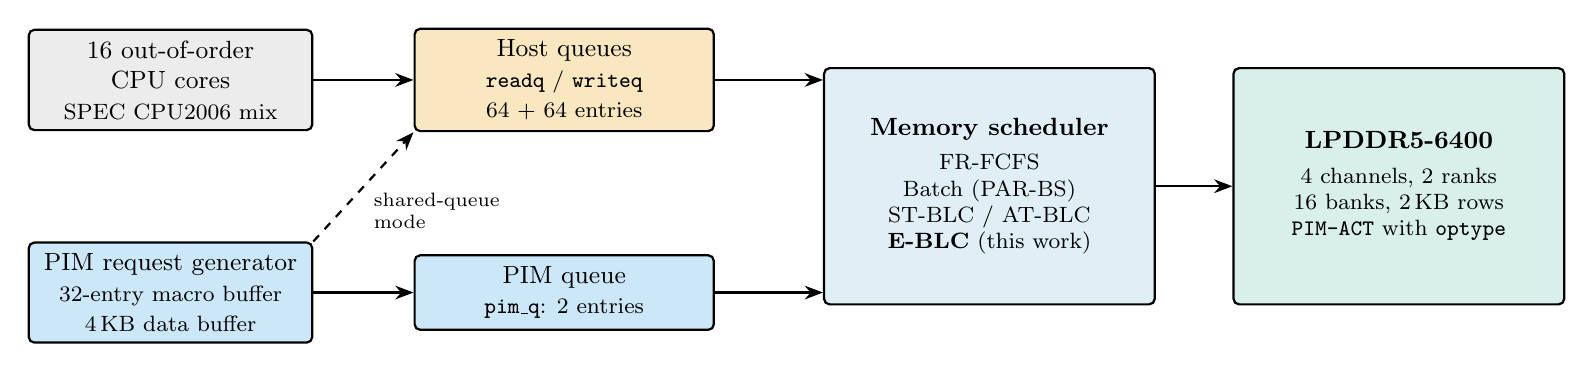
\begin{tikzpicture}[font=\small]
\node[box, fill=gray!15, minimum width=36mm] (cpu) at (0,2.2) {16 out-of-order\\CPU cores\\{\footnotesize SPEC CPU2006 mix}};
\node[box, fill=cOrange!25, minimum width=38mm] (hq) at (5.0,2.2) {Host queues\\{\footnotesize \cmd{readq} / \cmd{writeq}}\\{\footnotesize 64 + 64 entries}};
\node[box, fill=cSky!30, minimum width=36mm] (gen) at (0,-0.5) {PIM request generator\\{\footnotesize 32-entry macro buffer}\\{\footnotesize 4\,KB data buffer}};
\node[box, fill=cSky!30, minimum width=38mm] (pq) at (5.0,-0.5) {PIM queue\\{\footnotesize \cmd{pim\_q}: 2 entries}};
\node[box, font=\footnotesize, fill=cBlue!12, minimum width=42mm, minimum height=30mm] (sch) at (10.4,0.85) {\textbf{\small Memory scheduler}\\[3pt]FR-FCFS\\Batch (PAR-BS)\\\stblc{} / \atblc\\\textbf{\eblc} (this work)};
\node[box, font=\footnotesize, fill=cGreen!15, minimum width=42mm, minimum height=30mm] (dram) at (15.6,0.85) {\textbf{\small LPDDR5-6400}\\[3pt]4 channels, 2 ranks\\16 banks, 2\,KB rows\\\pimact{} with \cmd{optype}};
\draw[->, thick] (cpu) -- (hq);
\draw[->, thick] (gen) -- (pq);
\draw[->, thick] (hq.east) -- (hq.east -| sch.west);
\draw[->, thick] (pq.east) -- (pq.east -| sch.west);
\draw[->, thick] (sch) -- (dram);
\draw[->, thick, dashed] (gen.north east) -- (hq.south west) node[pos=0.52, below right=-1pt, font=\scriptsize, align=left]{shared-queue\\mode};
\end{tikzpicture}}
\caption{Memory subsystem modelled in Ramulator. In FR-FCFS and Batch mode PIM micro-requests merge into the shared host queue (dashed); the balancers use the dedicated 2-entry \cmd{pim\_q}.}\label{fig:arch}
\end{figure*}

\begin{figure*}[!t]
\centering
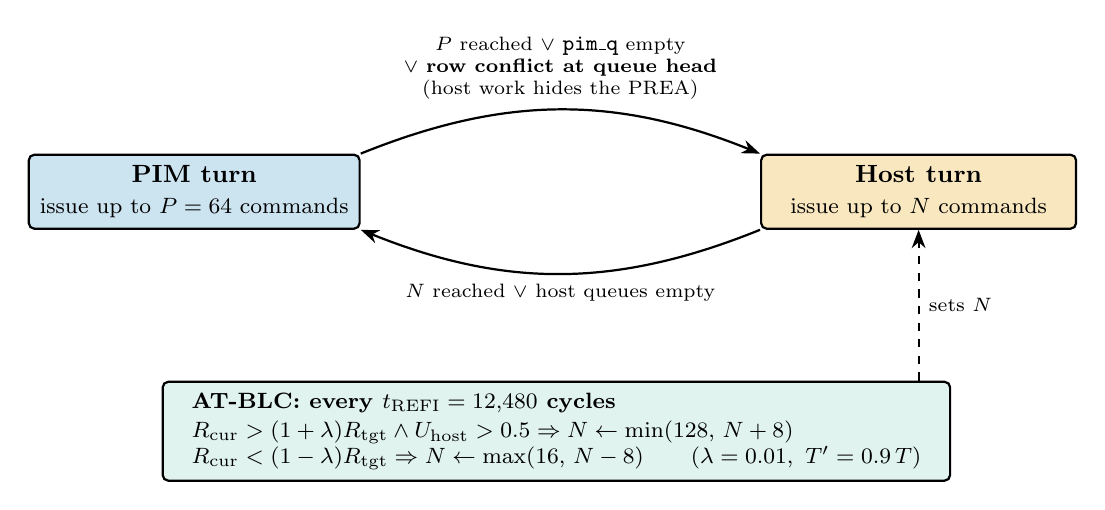
\begin{tikzpicture}[font=\small, node distance=8mm]
\node[box, fill=cBlue!20, minimum width=40mm] (pim) at (0,0) {\textbf{PIM turn}\\{\footnotesize issue up to $P=64$ commands}};
\node[box, fill=cOrange!25, minimum width=40mm] (host) at (9.2,0) {\textbf{Host turn}\\{\footnotesize issue up to $N$ commands}};
\draw[->, thick, bend left=22] (pim.north east) to node[above, align=center, font=\scriptsize]{$P$ reached\ $\vee$\ \cmd{pim\_q} empty\\$\vee$ \textbf{row conflict at queue head}\\(host work hides the PREA)} (host.north west);
\draw[->, thick, bend left=22] (host.south west) to node[below, align=center, font=\scriptsize]{$N$ reached\ $\vee$ host queues empty} (pim.south east);
\node[box, fill=cGreen!12, minimum width=100mm, anchor=north, align=left, font=\footnotesize] (at) at (4.6,-2.4)
 {\textbf{\atblc: every $\trefi=12{,}480$ cycles}\\[1pt]
  $R_{\mathrm{cur}}>(1+\lambda)R_{\mathrm{tgt}}\wedge U_{\mathrm{host}}>0.5 \Rightarrow N\leftarrow\min(128,\,N+8)$\\
  $R_{\mathrm{cur}}<(1-\lambda)R_{\mathrm{tgt}} \Rightarrow N\leftarrow\max(16,\,N-8)$\qquad ($\lambda=0.01,\ T'=0.9\,T$)};
\draw[->, thick, dashed] (at.north -| host.south) -- node[right, font=\scriptsize]{sets $N$} (host.south);
\end{tikzpicture}
\caption{Turn-switching logic of the throughput balancer. \stblc{} keeps $N=64$; \atblc{} updates $N\in[16,128]$ once per refresh interval.}\label{fig:balancer}
\end{figure*}

% =====================================================================
\section{Implementation and Experimental Methodology}\label{sec:method}

\subsection{Toolchain overview}
Two open-source cycle-level simulators are used, because the paper's claims live at two different levels:

\begin{itemize}
\item \textbf{Samsung PIMSimulator} (derived from DRAMSim2~\cite{dramsim2}) models the DRAM protocol and the bank-level SIMD FP16 units of HBM-PIM. It lets us execute real kernels and check results bit-exactly. Simulated at 1\,ns per cycle with 16 banks per rank (\cmd{system\_hbm\_64ch.ini}).
\item \textbf{Ramulator}~\cite{ramulator} models a full memory system with trace-driven out-of-order cores. It lets us measure interference between 16 host cores and a PIM stream under different schedulers.
\end{itemize}

\subsection{Part A: PIMSimulator changes}\label{sec:partA}
\begin{description}[leftmargin=0pt,labelindent=0pt,font=\bfseries]
\item[Command set.] \cmd{PIM\_ACT} added to \cmd{BusPacketType}; packets carry \cmd{isPIM} and an 8-bit \cmd{optype}. We fixed an upstream bug where the 8-argument \cmd{BusPacket} constructor omitted \cmd{bank(b)} from its initialiser list, leaving uninitialised bank IDs (observed values such as 32707) that triggered assertion failures.
\item[Optype ISA.] 35 optypes (\cref{tab:optype}); an explicit \cmd{NO\_OPTYPE = 0xFF} sentinel prevents optype~0 (\cmd{OP\_MUL\_GRF\_A\_BANK}) from being mistaken for ``unset''.
\item[Multi-bank execution.] \cmd{PIMRank::doPIMACT} activates all 16 banks and executes FP16 SIMD operations (MAC for GEMV, ADD, MUL, ReLU) on bank-pair units. \cmd{CommandQueue::isIssuable} refuses \pimact unless every bank is idle and past its $t_{RP}/t_{RRD}$ recovery; a PRECHARGE issued in \pimact mode closes all banks of the rank.
\item[Timing.] $t_{RCD,\pimact}=t_{RCD}+1$ cycle; $t_{RCDWR}$/$t_{RCDRD}$ enforced separately in \cmd{PimActTiming.h}. AAO scales $t_{RCD}$, $t_{RAS}$, $t_{RC}$, $t_{RP}$ by factors $0.5/0.6/0.6/0.5$ (floors 2/4/6/2 cycles) for register-only operations. These factors are \emph{our} assumption, exposed as \cmd{AAO\_TRCD}, \cmd{AAO\_TRAS}, \cmd{AAO\_TRC}, \cmd{AAO\_TRP}.
\item[PREA-aware scheduling.] Following the paper's \S5.1 principle that same-row, same-optype requests are row hits, \cmd{CommandQueue::process\_precharge} scans all 16 bank queues before issuing a rank-wide PRECHARGE and suppresses it if another bank still has a pending command on its open row (stopping at barrier packets). Enabled by default; \cmd{PIMACT\_PREA\_AWARE=0} restores naive per-bank precharge. The scan does not compare optypes; a diagnostic (\cmd{[B4-HIST]}) confirmed zero same-row optype collisions in all four benchmarks and was validated with an injected positive control.
\item[Verification.] Golden FP16 reference data (seed 1113) for the four kernels, plus an \emph{A3} test that runs each kernel under both the legacy and \pimact protocols and compares every output burst bitwise: \cmd{[A3-OK]}, 0 mismatches. The Google Test suite for the \pimact kernels passes 4/4.
\end{description}

\subsection{Part B: Ramulator changes}
\begin{description}[leftmargin=0pt,labelindent=0pt,font=\bfseries]
\item[LPDDR5-6400 model.] New \cmd{LPDDR5.h/.cpp}: 3200\,MHz bus ($t_{CK}=0.3125$\,ns), 16-bit channel, BL16 (32\,B per access), 8\,Gb die, 16 banks (4 bank groups $\times$ 4), 2\,KB rows. Timing in cycles: $nRCD{=}18$, $nRP{=}18$, $nRAS{=}42$, $nRC{=}60$, $nRTP{=}8$, $nWR{=}34$, $nFAW{=}16$, $nRRD{=}4$, $nRFC{=}140$, $nREFI{=}12480$.
\item[Requests and queues.] \cmd{Request} gains \cmd{is\_pim}, \cmd{optype}, \cmd{batch\_id} and distinct PIM read/write types. FR-FCFS and Batch place PIM and host requests in the \emph{same} queue; the balancers use host queues of 64 entries each and a dedicated 2-entry \cmd{pim\_q}. An embedded request generator (32-entry macro buffer, 4\,KB data buffer) expands a GEMV stream into micro-requests per rank, bank, row and column chunk.
\item[PREA accounting.] Rank-wide precharges issued when service switches between a PIM stream and the host are counted (\cmd{prea\_count}).
\item[Policies.] FR-FCFS; Batch (size 64, older batch first, FR-FCFS inside); \stblc{} ($P{=}N{=}64$, early turn switch on a PIM row conflict); \atblc{} (per-$\trefi$ update of $N$, 50\% slot rule, $\lambda{=}0.01$, $N_{\min,\max}{=}16,128$, $d{=}8$); and \eblc{} below.
\item[Trace parser.] CRLF/whitespace trimming added to \cmd{Processor.cpp}; upstream \cmd{stoul} threw on trailing \cmd{\textbackslash r}.
\end{description}

\subsection{Proposed scheduler: E-BLC}
ST-BLC and AT-BLC serialise turns at channel level, so host requests wait even when they touch banks the PIM stream is not using. \eblc{} (Elastic Bank-conflict-aware Balancer) adds two rules on top of the turn mechanism (\cref{fig:eblc}):
\begin{enumerate}
\item \textbf{BLP interleaving.} If the head PIM and host requests map to different bank groups, the host request is a row hit and the PIM request is not, the host request is issued immediately, without ending the PIM turn.
\item \textbf{Elastic quota lending.} During a PIM turn, if the PIM request would miss and a host row hit is ready, the PIM turn lends a slot to the host; the host turn's quota grows by the lent slots and is reset at the next switch.
\end{enumerate}

\begin{figure*}[!t]
\centering
\resizebox{\textwidth}{!}{%
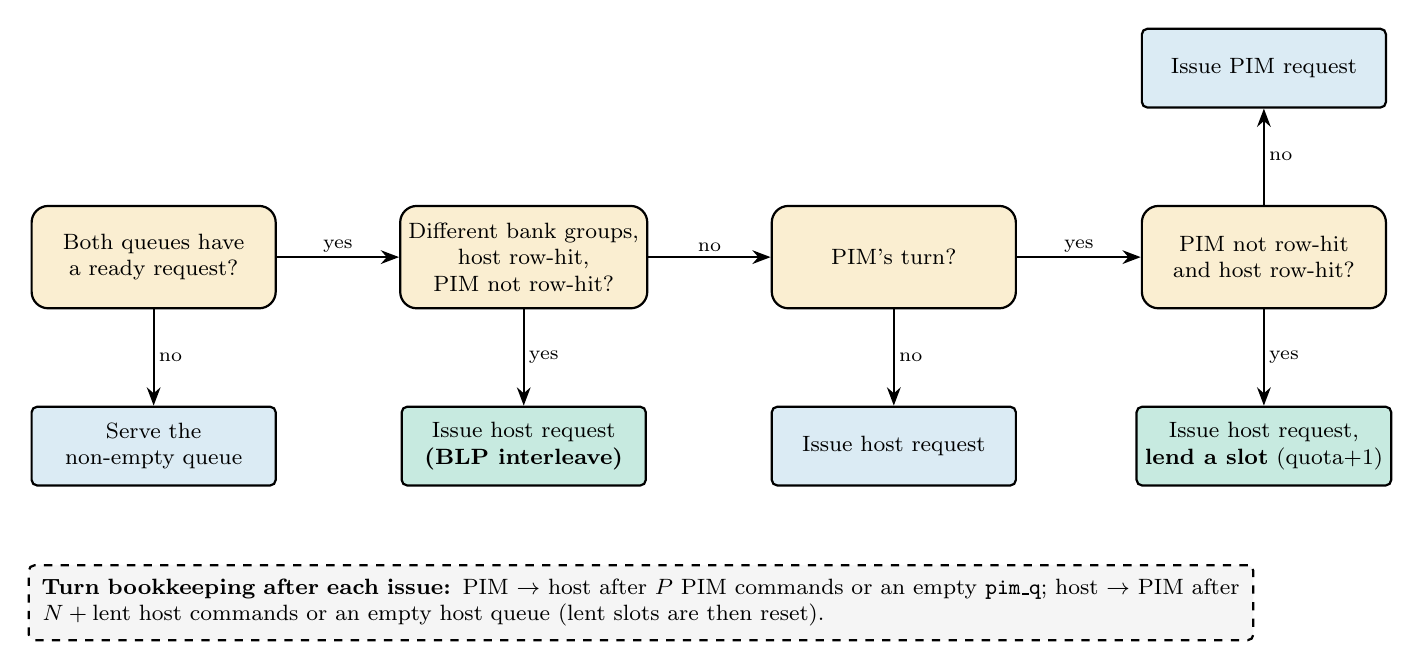
\begin{tikzpicture}[font=\footnotesize,
  dec/.style={draw, thick, rounded corners=6pt, fill=cOrange!18, align=center, inner sep=3pt, minimum width=31mm, minimum height=13mm},
  act/.style={draw, thick, rounded corners=2pt, fill=cBlue!14, align=center, inner sep=3pt, minimum width=31mm, minimum height=10mm},
  lbl/.style={font=\scriptsize, inner sep=1.5pt}]
\node[dec] (d1) at (0,3.0) {Both queues have\\a ready request?};
\node[dec] (d2) at (4.7,3.0) {Different bank groups,\\host row-hit,\\PIM not row-hit?};
\node[dec] (d3) at (9.4,3.0) {PIM's turn?};
\node[dec] (d4) at (14.1,3.0) {PIM not row-hit\\and host row-hit?};
\node[act] (a0) at (0,0.6) {Serve the\\non-empty queue};
\node[act, fill=cGreen!22] (a1) at (4.7,0.6) {Issue host request\\\textbf{(BLP interleave)}};
\node[act] (a2) at (9.4,0.6) {Issue host request};
\node[act, fill=cGreen!22] (a3) at (14.1,0.6) {Issue host request,\\\textbf{lend a slot} (quota+1)};
\node[act] (a4) at (14.1,5.4) {Issue PIM request};
\draw[->, thick] (d1) -- node[lbl, above]{yes} (d2);
\draw[->, thick] (d2) -- node[lbl, above]{no} (d3);
\draw[->, thick] (d3) -- node[lbl, above]{yes} (d4);
\draw[->, thick] (d1) -- node[lbl, right]{no} (a0);
\draw[->, thick] (d2) -- node[lbl, right]{yes} (a1);
\draw[->, thick] (d3) -- node[lbl, right]{no} (a2);
\draw[->, thick] (d4) -- node[lbl, right]{yes} (a3);
\draw[->, thick] (d4) -- node[lbl, right]{no} (a4);
\node[draw, thick, dashed, rounded corners=2pt, align=left, text width=15.2cm, inner sep=5pt, fill=gray!8, anchor=north west] at (-1.6,-0.9)
 {\textbf{Turn bookkeeping after each issue:} PIM $\to$ host after $P$ PIM commands or an empty \cmd{pim\_q}; host $\to$ PIM after $N+\text{lent}$ host commands or an empty host queue (lent slots are then reset).};
\end{tikzpicture}}
\caption{Decision flow of the proposed \eblc{} scheduler for one controller cycle. The two green boxes are the additions to the turn-based balancer.}\label{fig:eblc}
\end{figure*}

\subsection{Experimental setup}
\begin{table*}[!t]
\centering
\caption{Simulated system and workload configuration used for the Ramulator experiments.}\label{tab:config}
\footnotesize
\begin{tabular}{@{}p{3.2cm}p{13.8cm}@{}}
\toprule
\textbf{Component} & \textbf{Setting}\\
\midrule
Host & 16 out-of-order cores, one SPEC CPU2006 trace each: mcf, lbm, milc, leslie3d, soplex, GemsFDTD, libquantum, omnetpp, bzip2, zeusmp, gromacs, cactusADM, hmmer, sjeng, h264ref, xalancbmk. No cache model; 200\,k warm-up and 2\,M instructions per core limit.\\
Memory & LPDDR5-6400, 4 channels, 2 ranks/channel, 16 banks/rank, 2\,KB row, BL16, timing as in \cref{sec:method}.\\
Controller queues & \cmd{readq}=\cmd{writeq}=64; \cmd{pim\_q}=2 (balancers); macro buffer 32; data buffer 4\,KB.\\
PIM workload & GEMV micro-request stream, 65{,}536 micro-ops per channel (262{,}144 total, 32\,B each, 8\,MiB).\\
Balancer & $P=64$; $N_0=64$; $N\in[16,128]$; $d=8$; $\lambda=0.01$; $T=5\times10^{6}$ cycles, $T'=0.9\,T$.\\
Policies & Host-only, FR-FCFS, Batch (64), \stblc, \atblc, \eblc.\\
\bottomrule
\end{tabular}
\end{table*}

\paragraph{Metrics.} \emph{Aggregate host IPC} is total retired instructions of the 16 cores divided by total CPU cycles. \emph{Host slowdown} is $(\mathrm{IPC}_{\mathrm{host\text{-}only}}-\mathrm{IPC}_{\mathrm{co}})/\mathrm{IPC}_{\mathrm{host\text{-}only}}$. \emph{Weighted speedup} normalises per-core IPC to the host-only run. \emph{PIM bandwidth} is PIM bytes moved divided by total cycles, at 3.2\,GHz. \emph{PREA count} is the number of rank-wide precharges. The \emph{QoS ratio} is $T_{\mathrm{target}}/T_{\mathrm{actual}}$ with $T_{\mathrm{target}}=5\times10^6$ and $T_{\mathrm{actual}}$ the total simulated cycles; $\ge 1$ means the target is met. In Part A, \emph{gain} $=\text{Baseline cycles}/\text{PIM-ACT cycles}-1$, measured both over the PIM compute region and over the whole run (preload + region + readback).

\paragraph{Superseded earlier numbers.} Our first Ramulator prototype reported FR-FCFS/Batch slowdowns of 3.57\%/3.65\%. The final model puts PIM and host in one shared queue and counts PREA turnaround penalties; all results below use the final model, and the earlier numbers should not be compared with them.

% =====================================================================
\section{Baseline Results}\label{sec:baseline}

\subsection{Part A: legacy mode-switch protocol (HBM-PIM baseline)}
\Cref{tab:baseline-cycles} gives the baseline cycle counts of the four paper kernels. These are preserved exactly across all later changes (a regression check in our test matrix).

\begin{table}[!tbp]
\centering
\caption{Baseline (legacy mode-switch) protocol: cycle counts per execution phase (1\,cycle = 1\,ns).}\label{tab:baseline-cycles}
\scriptsize
\setlength{\tabcolsep}{3pt}
\begin{tabular}{@{}lrrrrr@{}}
\toprule
\textbf{Kernel} & \textbf{Preload} & \textbf{PIM region} & \textbf{Readback} & \textbf{Total} & \textbf{Preload share}\\
\midrule
GEMV (4K$\times$4K) & 44{,}283 & 13{,}483 & 157 & 57{,}923 & 76.5\%\\
ADD (1M)            & 4{,}242  & 3{,}308  & 2{,}076 & 9{,}626 & 44.1\%\\
MUL (2M)            & 8{,}482  & 6{,}286  & 4{,}512 & 19{,}280 & 44.0\%\\
ReLU (4M)           & 8{,}482  & 7{,}660  & 8{,}989 & 25{,}131 & 33.8\%\\
\bottomrule
\end{tabular}
\end{table}

\paragraph{Execution timeline.} The GEMV PIM region lasts 13{,}483 cycles (13.5\,$\mu$s), consistent with the paper's ``about 13\,$\mu$s'', but it is only 23.3\% of the run (\cref{fig:phases}). This matters for every whole-run comparison below.

\begin{figure*}[!t]
\centering
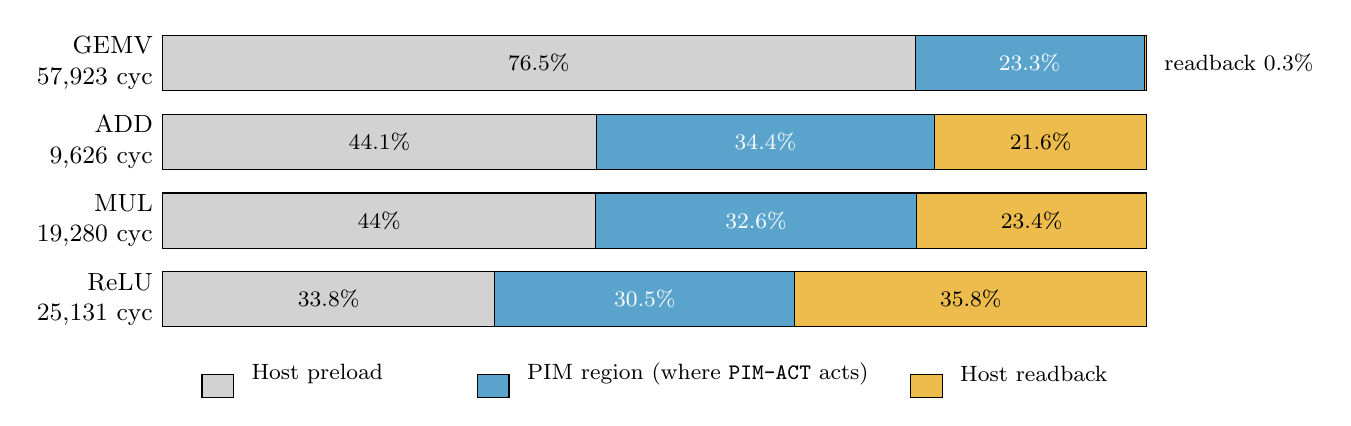
\begin{tikzpicture}[font=\small]
\newcommand{\phasebar}[5]{%
 \pgfmathsetmacro{\tot}{#3+#4+#5}
 \pgfmathsetmacro{\wa}{12.5*#3/\tot}
 \pgfmathsetmacro{\wb}{12.5*(#3+#4)/\tot}
 \pgfmathsetmacro{\pa}{100*#3/\tot}
 \pgfmathsetmacro{\pb}{100*#4/\tot}
 \pgfmathsetmacro{\pc}{100*#5/\tot}
 \draw[fill=gray!35] (0,#1) rectangle (\wa,#1+0.7);
 \draw[fill=cBlue!65] (\wa,#1) rectangle (\wb,#1+0.7);
 \draw[fill=cOrange!70] (\wb,#1) rectangle (12.5,#1+0.7);
 \node[left, align=right] at (0,#1+0.35) {#2};
 \node[font=\footnotesize] at (\wa/2,#1+0.35) {\pgfmathprintnumber[fixed,precision=1]{\pa}\%};
 \node[font=\footnotesize, text=white] at (\wa+0.5*\wb-0.5*\wa,#1+0.35) {\pgfmathprintnumber[fixed,precision=1]{\pb}\%};
 \pgfmathparse{int(#5/\tot>0.08)}
 \ifnum\pgfmathresult=1
   \node[font=\footnotesize] at (\wb+0.5*12.5-0.5*\wb,#1+0.35) {\pgfmathprintnumber[fixed,precision=1]{\pc}\%};
 \else
   \node[font=\footnotesize, anchor=west] at (12.6,#1+0.35) {readback \pgfmathprintnumber[fixed,precision=1]{\pc}\%};
 \fi
}
\phasebar{3.0}{GEMV\\57{,}923 cyc}{44.283}{13.483}{0.157}
\phasebar{2.0}{ADD\\9{,}626 cyc}{4.242}{3.308}{2.076}
\phasebar{1.0}{MUL\\19{,}280 cyc}{8.482}{6.286}{4.512}
\phasebar{0.0}{ReLU\\25{,}131 cyc}{8.482}{7.660}{8.989}
\draw[fill=gray!35] (0.5,-0.9) rectangle (0.9,-0.6) node[right=3pt, font=\footnotesize]{Host preload};
\draw[fill=cBlue!65] (4.0,-0.9) rectangle (4.4,-0.6) node[right=3pt, font=\footnotesize]{PIM region (where \pimact acts)};
\draw[fill=cOrange!70] (9.5,-0.9) rectangle (9.9,-0.6) node[right=3pt, font=\footnotesize]{Host readback};
\end{tikzpicture}
\caption{Share of each baseline run spent in host preload, the PIM compute region and host readback (drawn to scale). \pimact can only change the middle segment.}\label{fig:phases}
\end{figure*}

\paragraph{Mode-switch cost.} We instrumented the memory controller with cycle timestamps (\cmd{[MODE-SWITCH]} tags) and analysed them with \cmd{analyze\_mode\_switch.py}. \Cref{tab:modeswitch} breaks the round trip into its phases; \cref{fig:modeswitch} shows the totals.

\begin{table*}[!t]
\centering
\caption{Measured phases of the legacy mode-switch round trip (GEMV window; ADD differs by $\le1$ cycle). Bus packets: 4{,}864 in total.}\label{tab:modeswitch}
\footnotesize
\begin{tabular}{@{}llrrl@{}}
\toprule
\textbf{\#} & \textbf{Phase} & \textbf{Cycles} & \textbf{Packets} & \textbf{Function}\\
\midrule
1 & \cmd{parkIn()}            & 87 & 2048 & row-parking reads across all 16 banks\\
2 & SB $\to$ HAB              & 41 & 256  & mode-register writes (\cmd{PIM\_ABMR\_RA})\\
3 & HAB $\to$ HAB-PIM         & 11 & 128  & reset PIM program counter\\
4 & PIM compute               & 13{,}132 & --- & arithmetic execution\\
5 & HAB-PIM $\to$ HAB         & 11 & 128  & write to \cmd{pim\_reg\_ra\_}\\
6 & HAB $\to$ SB              & 22 & 256  & mode-register writes (\cmd{PIM\_SBMR\_RA})\\
7 & \cmd{parkOut()}           & 86 & 2048 & row-parking reads across all 16 banks\\
\midrule
\multicolumn{2}{l}{Entry overhead (1--3, incl.\ gaps)} & 167 & & GEMV; ADD 168\\
\multicolumn{2}{l}{Exit overhead (5--7, incl.\ gaps)}  & 184 & & all kernels\\
\multicolumn{2}{l}{\textbf{Round trip}} & \textbf{351} & & ADD 352\,ns; paper: ``about 350\,ns''\\
\bottomrule
\end{tabular}
\end{table*}

\begin{figure}[!tbp]
\centering
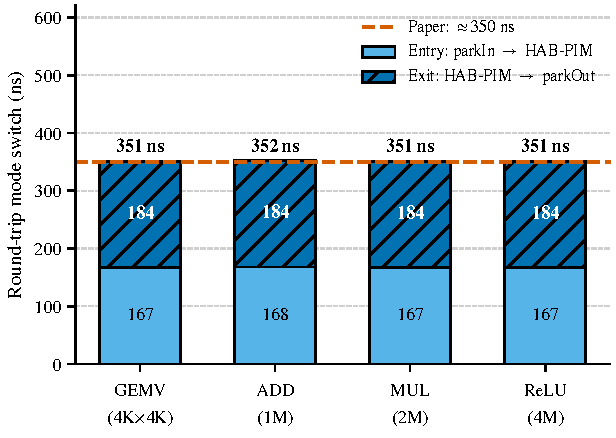
\includegraphics[width=\columnwidth]{figs/fig_mode_switch.pdf}
\caption{Measured round-trip mode-switch cost of the baseline protocol for the four kernels, split into entry and exit; the dashed line is the paper's estimate.}\label{fig:modeswitch}
\end{figure}

\begin{figure*}[!t]
\centering
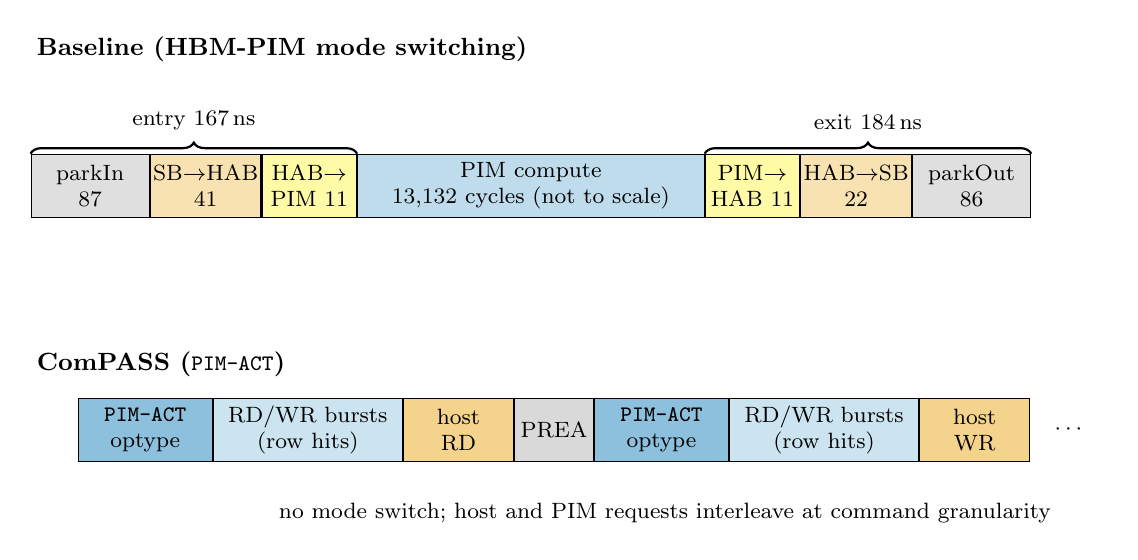
\begin{tikzpicture}[font=\footnotesize]
\node[anchor=south west, font=\small\bfseries] at (-0.5,3.45) {Baseline (HBM-PIM mode switching)};
\node[seg, fill=gray!25, minimum width=15mm] (a1) at (0.3,2.0) {parkIn\\87};
\node[seg, fill=cOrange!30, minimum width=14mm, right=0pt of a1] (a2) {SB$\to$HAB\\41};
\node[seg, fill=yellow!35, minimum width=12mm, right=0pt of a2] (a3) {HAB$\to$\\PIM\ 11};
\node[seg, fill=cBlue!25, minimum width=44mm, right=0pt of a3] (a4) {PIM compute\\13{,}132 cycles (not to scale)};
\node[seg, fill=yellow!35, minimum width=12mm, right=0pt of a4] (a5) {PIM$\to$\\HAB\ 11};
\node[seg, fill=cOrange!30, minimum width=14mm, right=0pt of a5] (a6) {HAB$\to$SB\\22};
\node[seg, fill=gray!25, minimum width=15mm, right=0pt of a6] (a7) {parkOut\\86};
\draw[decorate, decoration={brace, amplitude=4pt}, thick] (a1.north west) -- (a3.north east) node[midway, above=5pt]{entry 167\,ns};
\draw[decorate, decoration={brace, amplitude=4pt}, thick] (a5.north west) -- (a7.north east) node[midway, above=5pt]{exit 184\,ns};
\node[anchor=south west, font=\small\bfseries] at (-0.5,-0.55) {ComPASS (\pimact)};
\node[seg, fill=cBlue!45, minimum width=17mm] (b1) at (1.0,-1.1) {\cmd{PIM-ACT}\\optype};
\node[seg, fill=cBlue!20, minimum width=24mm, right=0pt of b1] (b2) {RD/WR bursts\\(row hits)};
\node[seg, fill=cOrange!45, minimum width=14mm, right=0pt of b2] (b3) {host\\RD};
\node[seg, fill=gray!30, minimum width=10mm, right=0pt of b3] (b4) {PREA};
\node[seg, fill=cBlue!45, minimum width=17mm, right=0pt of b4] (b5) {\cmd{PIM-ACT}\\optype};
\node[seg, fill=cBlue!20, minimum width=24mm, right=0pt of b5] (b6) {RD/WR bursts\\(row hits)};
\node[seg, fill=cOrange!45, minimum width=14mm, right=0pt of b6] (b7) {host\\WR};
\node[seg, fill=white, draw=none, minimum width=10mm, right=0pt of b7] (b8) {$\cdots$};
\node[font=\footnotesize, align=center] at (7.6,-2.15) {no mode switch; host and PIM requests interleave at command granularity};
\end{tikzpicture}
\caption{Command timelines. The baseline protocol stalls normal traffic for the 351\,ns entry and exit sequences; \pimact removes them.}\label{fig:protocol}
\end{figure*}

\subsection{Part B: host-only and shared-queue baselines}
The reference point for all slowdowns is the \emph{host-only} run: 16 cores, no PIM stream, aggregate IPC 14.0967 in 7{,}985{,}629 cycles. Adding the PIM GEMV stream under the two shared-queue baselines (FR-FCFS, Batch) gives \cref{tab:baseline-ram} and \cref{fig:baseline-ram}.

\begin{table*}[!t]
\centering
\caption{Ramulator baselines: host-only, FR-FCFS and Batch (PAR-BS, batch 64), 16 cores + 262{,}144 PIM micro-ops.}\label{tab:baseline-ram}
\footnotesize
\begin{tabular}{@{}lrrrrrrr@{}}
\toprule
\textbf{Policy} & \textbf{Host IPC} & \textbf{Slowdown} & \textbf{WS} & \textbf{PIM BW} & \textbf{PREA} & \textbf{QoS} & \textbf{Cycles}\\
 & & (\%) & & (GB/s) & ($\times10^3$) & ratio & ($\times10^6$)\\
\midrule
Host-only & 14.0967 & 0 (ref.) & 1.0000 & --- & 2.5 & --- & 7.986\\
FR-FCFS   & 13.3931 & 4.99 & 0.9470 & 3.130 & 116.7 & 0.583 & 8.577\\
Batch     & 13.4018 & 4.93 & 0.9478 & 3.126 & 117.0 & 0.582 & 8.588\\
\bottomrule
\end{tabular}
\end{table*}

\begin{figure*}[!t]
\centering
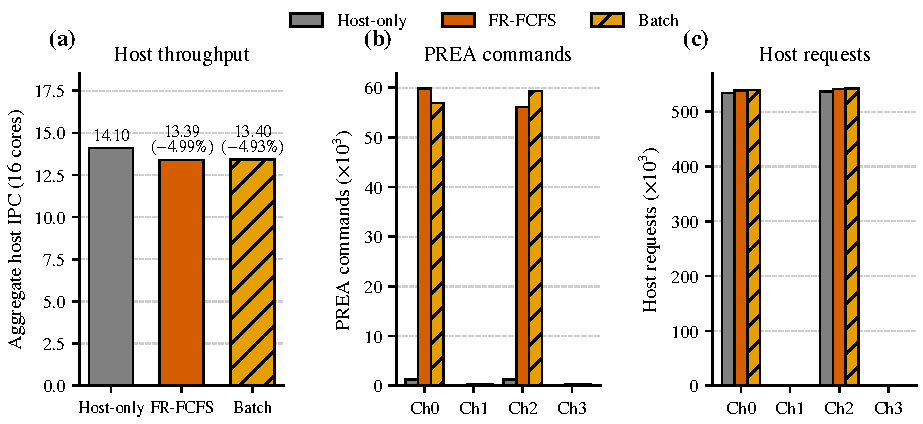
\includegraphics[width=\textwidth]{figs/fig_baseline_ramulator.pdf}
\caption{Baseline results. (a)~Aggregate host IPC of the 16 cores; (b)~rank-wide PREA commands per channel; (c)~host requests per channel. Host traffic reaches only channels 0 and 2 (address mapping of the trace set), while PIM spreads evenly over all four.}\label{fig:baseline-ram}
\end{figure*}

\paragraph{Observations.}
\begin{itemize}
\item Sharing a queue with the PIM stream costs the host about 5\% of its IPC. Batch scheduling changes this by only 0.06\,pp (4.93\% vs 4.99\%): grouping requests does not protect the host from a streaming PIM client.
\item PREA commands jump from 2.5\,k (host-only) to $\approx$117\,k, almost all on channels 0 and 2 where host and PIM share banks (\cref{fig:baseline-ram}b). Channels 1 and 3 carry only PIM and need 367--370 PREAs each. This is the turnaround penalty the balancers try to hide.
\item PIM bandwidth is 3.13\,GB/s (0.78\,GB/s per channel) for both baselines, with a PIM row-hit rate of 98.2--98.4\%, so the PIM stream itself is not suffering from row thrashing; the host pays for the interleaving.
\item The QoS ratio is 0.58: with $T_{\mathrm{target}}=5\times10^6$ cycles, no policy, including the baselines, meets the target in this configuration (see limitations, \cref{sec:discussion}).
\end{itemize}

% =====================================================================
\section{Results of the Proposed Mechanisms}\label{sec:results}

\subsection{Part A: \pimact protocol}

\paragraph{Functional correctness.} All four kernels produce bit-identical FP16 results under \pimact and the legacy protocol (\cmd{[A3-OK]}, 0 mismatches over 4{,}096 / 1{,}048{,}576 / 2{,}097{,}152 / 4{,}194{,}304 outputs). No activation took the optype-collision path (\cmd{[B4-HIST] total=0}).

\paragraph{Speed-up versus the baseline protocol.} \Cref{tab:parta} and \cref{fig:fig7} compare PREA-aware \pimact (our headline configuration) with the baseline, over the PIM region and over the whole run, alongside the paper's targets.

\begin{table*}[!t]
\centering
\caption{\pimact versus the baseline protocol (cycles; gain $=$ baseline/\pimact $-1$). ``Paper'' values are those stated in the paper's text (\S6, Figure~7).}\label{tab:parta}
\footnotesize
\setlength{\tabcolsep}{4pt}
\begin{tabular}{@{}l r rr rr rr rr@{}}
\toprule
 & \textbf{Base} & \multicolumn{2}{c}{\textbf{AAO off}} & \multicolumn{2}{c}{\textbf{AAO on}} & \multicolumn{2}{c}{\textbf{Paper}} & \multicolumn{2}{c}{\textbf{Naive PREA}}\\
\cmidrule(lr){3-4}\cmidrule(lr){5-6}\cmidrule(lr){7-8}\cmidrule(l){9-10}
\textbf{Kernel} & \textbf{total} & total & region & total & region & off & on & total & region\\
\midrule
GEMV & 57{,}923 & 57{,}567 & $+3.25$ & 57{,}189 & $+6.32$ & $+2.54$ & $+9.65$ & 71{,}033 & $-49.1$\\
ADD  & 9{,}626  & 9{,}468  & $+7.16$ & 9{,}468  & $+7.16$ & $+9.68$ & $+10.00$ & 11{,}602 & $-31.3$\\
MUL  & 19{,}280 & 19{,}194 & $+2.36$ & 19{,}194 & $+2.36$ & $+11.38$ & $+11.53$ & 23{,}080 & $-37.2$\\
ReLU & 25{,}131 & 25{,}809 & $-2.75$ & 25{,}809 & $-2.75$ & $+4.51$ & $+4.65$ & 30{,}903 & $-42.7$\\
\midrule
\multicolumn{10}{@{}l}{\textbf{Whole-run gain (\%)}:\quad
GEMV $+0.62$ / $+1.28$ (AAO off / on);\quad ADD $+1.67$;\quad MUL $+0.45$;\quad ReLU $-2.63$.}\\
\bottomrule
\end{tabular}
\end{table*}

\begin{figure*}[!t]
\centering
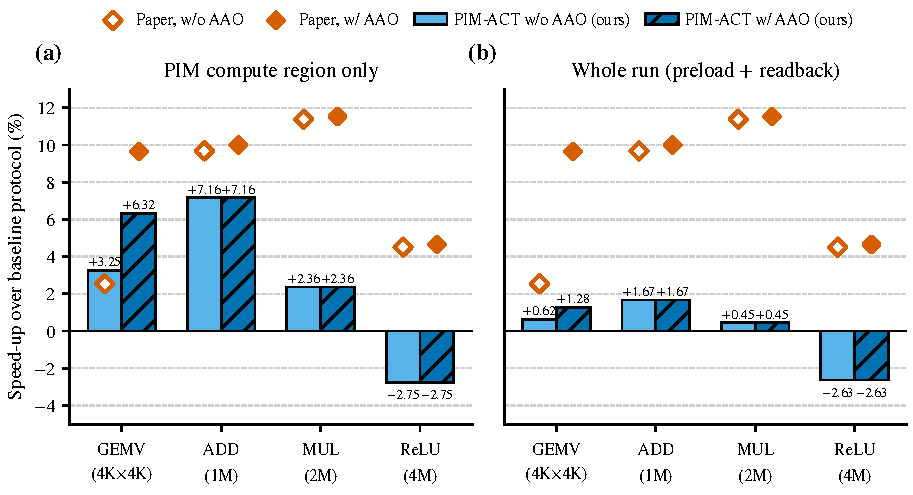
\includegraphics[width=\textwidth]{figs/fig_fig7.pdf}
\caption{Reproduction of the paper's Figure~7 speed-ups: (a)~over the PIM compute region only, (b)~over the whole run. Bars are ours; diamonds are the paper's targets.}\label{fig:fig7}
\end{figure*}

\begin{itemize}
\item \textbf{GEMV, AAO off} reproduces the paper's $+2.54\%$ to within 0.71\,pp when measured over the PIM region ($+3.25\%$). A back-of-envelope check agrees: removing one 351-cycle round trip from a 13{,}483-cycle region predicts $+2.67\%$.
\item \textbf{GEMV, AAO on} reaches $+6.32\%$ against the paper's $+9.65\%$. A runtime histogram (\cmd{[AAO-HIST]}) shows that only the 2{,}048 host-to-register moves (optype 32, about a third of the \pimact commands) qualify for the shortened timing; this accounts for the 378-cycle gain. Presumably the remaining activations read bank data and keep full timing (we did not histogram GEMV by optype).
\item \textbf{ADD, MUL} gain $+7.16\%$ and $+2.36\%$, below the paper's roughly 10--11\%. For these kernels the AAO branch never fired (\cmd{[AAO-HIST] total=0}): every operation reads a bank and needs full bitline timing, so AAO on/off are identical. We do not know whether the paper's AAO also covers bank-sourced operations.
\item \textbf{ReLU} is slower than baseline, the opposite of the paper's $+4.5\%$. \Cref{sec:relu} traces this to host readback.
\item Whole-run gains are 0.45--1.67\% for the three positive kernels because 44--77\% of each run is host preload outside the \pimact region. Our earlier whole-run-only measurement ($+0.62\%$ for GEMV) is what first looked like a failed reproduction.
\end{itemize}

\subsection{PREA-aware scheduling and phase breakdown}
Naive per-bank precharging closes rows that other banks still need; every kernel then pays for repeated \pimact activations and loses 16--19\% over the whole run. PREA-aware scheduling avoids this (\cref{fig:cmd-counts,fig:phase-breakdown}, \cref{tab:cmdcounts}).

\begin{table}[!tbp]
\centering
\caption{Command counts under naive per-bank precharge and PREA-aware scheduling (AAO off).}\label{tab:cmdcounts}
\scriptsize
\setlength{\tabcolsep}{3pt}
\begin{tabular}{@{}lrrrrrr@{}}
\toprule
 & \multicolumn{3}{c}{\textbf{\#\pimact}} & \multicolumn{3}{c}{\textbf{\#PRECHARGE}}\\
\cmidrule(lr){2-4}\cmidrule(l){5-7}
\textbf{Kernel} & naive & aware & change & naive & aware & change\\
\midrule
GEMV & 32{,}896 & 6{,}400 & $-80.5\%$ & 66{,}880 & 40{,}384 & $-39.6\%$\\
ADD  & 6{,}144  & 3{,}136 & $-49.0\%$ & 35{,}776 & 31{,}744 & $-11.3\%$\\
MUL  & 12{,}288 & 6{,}208 & $-49.5\%$ & 70{,}656 & 64{,}576 & $-8.6\%$\\
ReLU & 16{,}384 & 8{,}256 & $-49.6\%$ & 79{,}872 & 72{,}640 & $-9.1\%$\\
\bottomrule
\end{tabular}
\end{table}

\begin{figure*}[!t]
\centering
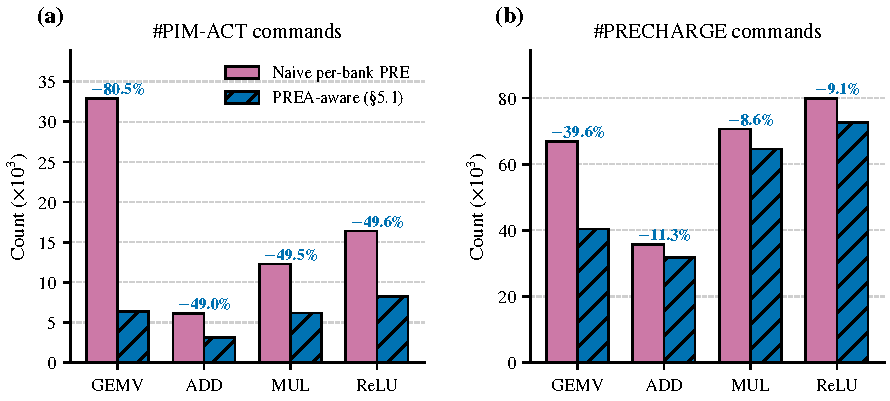
\includegraphics[width=0.92\textwidth]{figs/fig_cmd_counts.pdf}
\caption{Effect of PREA-aware scheduling on (a)~\pimact and (b)~PRECHARGE command counts relative to naive per-bank precharge.}\label{fig:cmd-counts}
\end{figure*}

\begin{figure*}[!t]
\centering
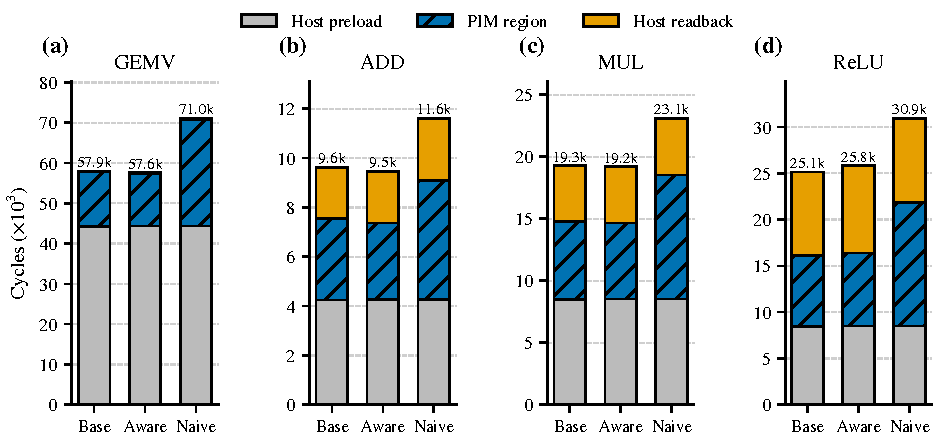
\includegraphics[width=\textwidth]{figs/fig_phase_breakdown.pdf}
\caption{Cycle breakdown per kernel: baseline, PREA-aware \pimact and naive-precharge \pimact (labels give total cycles). Relative to the baseline, the naive variant inflates the PIM region by 1.5--2.0$\times$.}\label{fig:phase-breakdown}
\end{figure*}

\subsection{Root cause of the ReLU slowdown}\label{sec:relu}
Under PREA-aware \pimact, ReLU needs 678 more cycles than the baseline ($25{,}809$ vs $25{,}131$). Decomposing by phase:
\begin{center}
\small
\begin{tabular}{@{}lrr@{}}
\toprule
\textbf{Phase} & \textbf{Extra cycles} & \textbf{Share}\\
\midrule
Host readback & 428 & 63.1\%\\
PIM region & 217 & 32.0\%\\
Preload / pipeline drain & 33 & 4.9\%\\
\midrule
\textbf{Total} & \textbf{678} & 100\%\\
\bottomrule
\end{tabular}
\end{center}
Readback dominates: PREA-aware scheduling deliberately keeps rows open across the rank, so when the host then reads the results it hits open rows belonging to other data and incurs 896 extra bank-conflict \cmd{ACT}s (64{,}384 vs 63{,}488). In the PIM region itself, the baseline alternates activations across even/odd bank pairs so that one pair's activation overlaps the other's compute, whereas rank-wide \pimact opens all 16 banks together and cannot pipeline this way. Both effects are inherent to the model we implemented; the paper does not report ReLU in enough detail to tell whether its \pimact variant avoids them.

\subsection{Part B: scheduling results}

\Cref{tab:main} and \cref{fig:eval4} give the main co-execution results for all six configurations.

\begin{table*}[!t]
\centering
\caption{Co-execution results: 16 cores + PIM GEMV stream on 4-channel LPDDR5-6400. Bold marks the best co-execution value in a column.}\label{tab:main}
\footnotesize
\begin{tabular}{@{}lrrrrrrr@{}}
\toprule
\textbf{Policy} & \textbf{Host IPC} & \textbf{Slowdown} & \textbf{WS} & \textbf{PIM BW} & \textbf{PREA} & \textbf{QoS} & \textbf{Cycles}\\
 & & (\%) & & (GB/s) & ($\times10^3$) & ratio & ($\times10^6$)\\
\midrule
Host-only & 14.0967 & 0 (ref.) & 1.0000 & --- & 2.5 & --- & 7.986\\
FR-FCFS   & 13.3931 & 4.99 & 0.9470 & 3.130 & \textbf{116.7} & 0.583 & 8.577\\
Batch     & 13.4018 & 4.93 & 0.9478 & 3.126 & 117.0 & 0.582 & 8.588\\
\stblc    & 13.5636 & 3.78 & 0.9541 & \textbf{3.162} & 152.7 & \textbf{0.589} & \textbf{8.489}\\
\atblc    & \textbf{13.6055} & \textbf{3.49} & \textbf{0.9565} & 3.124 & 151.0 & 0.582 & 8.593\\
\eblc{} (ours) & 13.5623 & 3.79 & 0.9513 & 3.140 & 152.0 & 0.585 & 8.548\\
\bottomrule
\end{tabular}
\end{table*}

\begin{figure*}[!t]
\centering
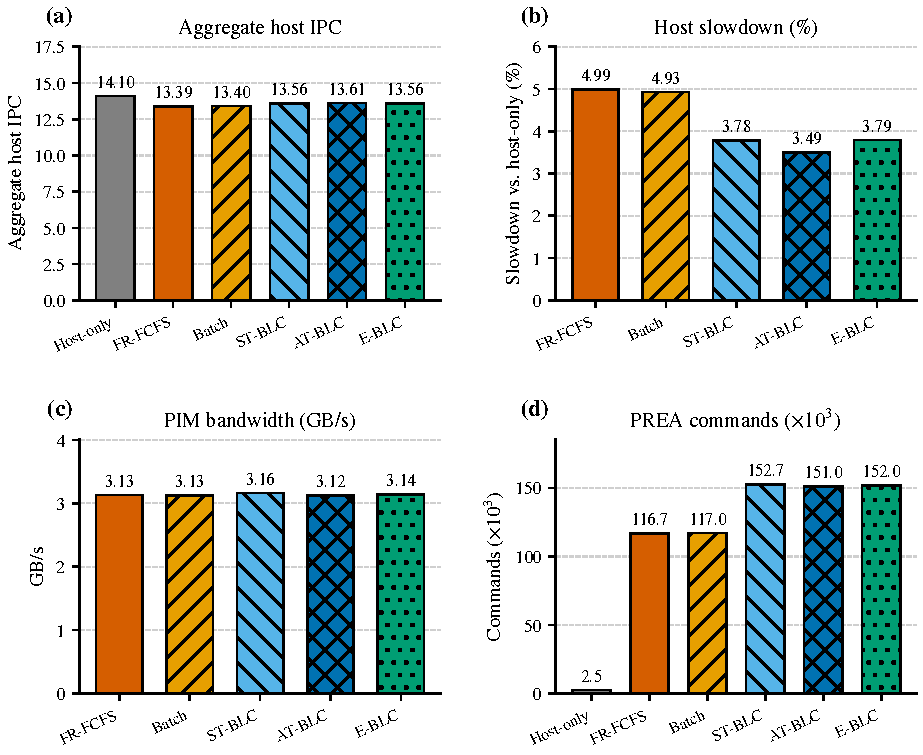
\includegraphics[width=0.93\textwidth]{figs/fig_eval4.pdf}
\caption{Full-system evaluation on 16 out-of-order cores and 4-channel LPDDR5-6400: (a)~aggregate host IPC, (b)~host slowdown versus the host-only run, (c)~PIM effective bandwidth, (d)~rank-wide PREA commands.}\label{fig:eval4}
\end{figure*}

\paragraph{Host protection.} Relative to FR-FCFS, \atblc{} raises aggregate IPC by 1.59\% and cuts slowdown by 30\% (4.99\% $\to$ 3.49\%); \stblc{} gives $+1.27\%$ IPC (24\% lower slowdown) and \eblc{} $+1.26\%$ (24\%). Batch is indistinguishable from FR-FCFS. This is the paper's qualitative claim: dedicating a shallow PIM queue and alternating turns bounds host damage.

\paragraph{PIM throughput.} PIM bandwidth stays within 3.12--3.16\,GB/s for all policies (spread $\le1.3\%$), so protecting the host did not cost PIM throughput. Because every policy serves the same 262{,}144 micro-ops at the same rate, ``PIM speedup'' relative to FR-FCFS is 1.00--1.01$\times$, i.e.\ no meaningful difference.

\paragraph{PREA commands rise.} The balancers issue 29--31\% \emph{more} PREA commands than FR-FCFS (\cref{fig:prea-qos}a). This is consistent with switching turns on every PIM row conflict, which ends PIM bursts earlier and so creates more PIM-to-host transitions. The gain is therefore not fewer precharges but precharge latency overlapped with host work, which shows up as lower host slowdown. Our figure is labelled ``PREA command count versus FR-FCFS'' because we cannot claim ``PREA elimination''.

\paragraph{QoS ratio and run length.} The ratio $T_{\mathrm{target}}/T_{\mathrm{actual}}$ is 0.58--0.59 for every policy (\cref{fig:prea-qos}b). Since $T_{\mathrm{actual}}$ is total simulated cycles, which also depend on when the slowest host core finishes, it is not a clean PIM-completion metric. \stblc{} finishes first (8.489\,M cycles, 1.0\% shorter than FR-FCFS); \atblc{} has the best IPC yet the longest run (8.593\,M), because IPC and run length weigh instructions retired by faster cores differently.

\begin{figure*}[!t]
\centering
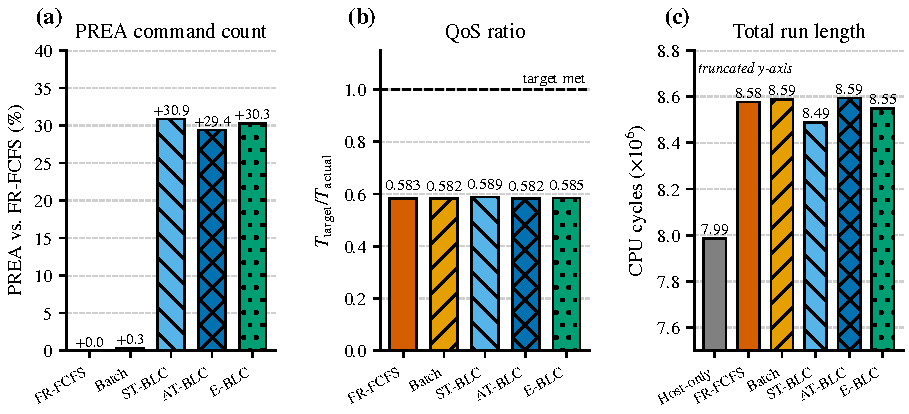
\includegraphics[width=\textwidth]{figs/fig_prea_qos.pdf}
\caption{(a)~PREA commands relative to FR-FCFS (positive $=$ more PREA), (b)~QoS ratio $T_{\mathrm{target}}/T_{\mathrm{actual}}$ (dashed line: target met), (c)~total run length (y-axis truncated).}\label{fig:prea-qos}
\end{figure*}

\subsection{Adaptive quota behaviour of AT-BLC}
\Cref{fig:nadapt} shows $N(t)$ for channel~0 (all four channels logged identical timelines). It starts at 56, drops by 8 per epoch to $N_{\min}=16$ within 0.08\,M cycles, as PIM is initially behind its target rate, stays there for $\approx$0.7\,M cycles, then climbs to $N_{\max}=128$ by 0.96\,M cycles when PIM runs ahead and the host used more than half its previous quota. It holds 128 for $\approx$1.8\,M cycles, falls back to 16 around 2.9\,M, and remains there to the last logged epoch (4.9\,M). Of the 392 logged epochs, 219 sit at 16 and 142 at 128; only 31 are transitional. \atblc{} thus behaves as a slow bang-bang controller with long plateaus, not a smoothly tracking one.

\begin{figure*}[!t]
\centering
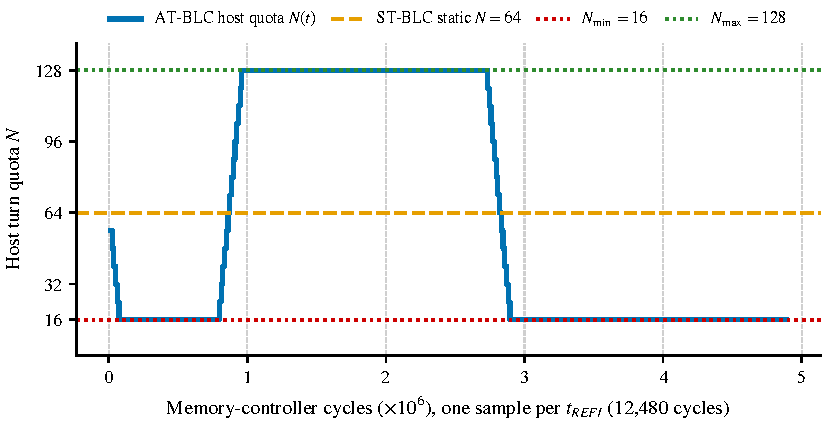
\includegraphics[width=0.85\textwidth]{figs/fig_N_adapt.pdf}
\caption{AT-BLC host turn quota $N(t)$ (channel~0) with the static $N=64$ of \stblc{} and the bounds $N_{\min}=16$, $N_{\max}=128$; one sample per $\trefi$.}\label{fig:nadapt}
\end{figure*}

\subsection{Proposed E-BLC}
\eblc{} lands at 3.79\% slowdown, essentially equal to \stblc{} (3.78\%), 0.30\,pp behind \atblc, and at 3.14\,GB/s PIM bandwidth; it issues 152.0\,k PREAs. We therefore \emph{cannot} claim that BLP interleaving and quota lending improve on the paper's balancers in this setup. Plausible reasons, which we have not tested: (i)~host traffic occupies only two of four channels, limiting concurrent cross-bank-group opportunities; (ii)~the GEMV stream hits 98\% row-hit rate, so PIM rarely conflicts and there is little quota to lend; (iii)~\eblc{} has no adaptive $N$. Note that an earlier plotting script in the repository contains hard-coded placeholder numbers that show \eblc{} at 2.92\% slowdown; they are used only if the CSV is missing and were \emph{not} measured. All numbers in this report come from \cmd{compass\_evaluation\_metrics.csv}.

\subsection{N:P parameter sweep (inconclusive)}\label{sec:sweep}
We attempted to mirror the paper's sensitivity study by sweeping the requested host quota $N\in\{16,32,64,96,128\}$ with $P=64$ for \stblc, \atblc{} and \eblc{}. \Cref{fig:sweep} shows every curve flat: results are identical for all $N$. The reason is in our code, not the architecture: the controller initialises \cmd{N\_limit} to 64 and never reads $N$ from the configuration file, and \cmd{parameter\_sweep.py} accepts \cmd{n\_limit} but never writes it to the generated config. The sweep also used a shortened setup (1\,M instructions, 32{,}768 PIM micro-ops, $T=3\times10^6$), so its absolute values (IPC $\approx$13.1, $\approx$4.2\,M cycles) are not comparable with \cref{tab:main}. We report the figure as a negative result and list the fix under future work; no sensitivity conclusion should be drawn from it.

\begin{figure*}[!t]
\centering
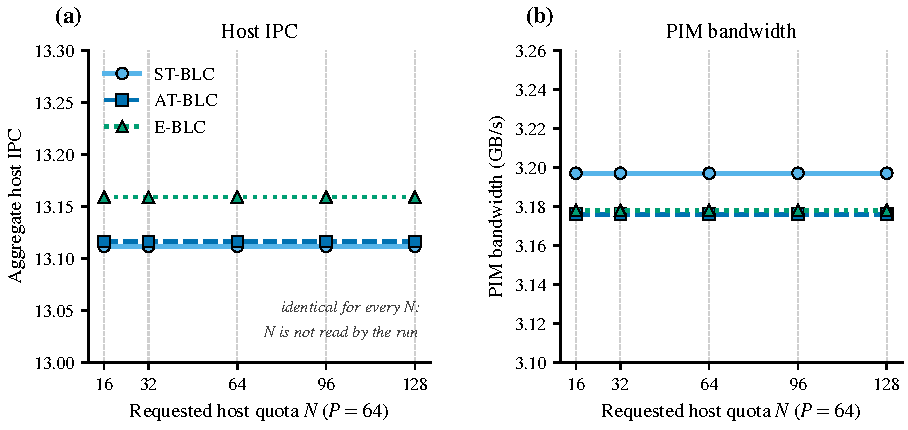
\includegraphics[width=0.92\textwidth]{figs/fig_sweep.pdf}
\caption{N:P sweep (shortened configuration). Flat lines show that the requested $N$ had no effect on the run.}\label{fig:sweep}
\end{figure*}

% =====================================================================
\section{Discussion}\label{sec:discussion}

\subsection{Comparison with the paper}
\begin{table*}[!t]
\centering
\caption{Reproduction status of the main claims.}\label{tab:status}
\footnotesize
\begin{tabularx}{\textwidth}{@{}>{\raggedright\arraybackslash}p{4.1cm}>{\raggedright\arraybackslash}X>{\raggedright\arraybackslash}p{3.1cm}@{}}
\toprule
\textbf{Claim (paper)} & \textbf{Our measurement} & \textbf{Status}\\
\midrule
Mode-switch round trip $\approx$350\,ns & 351--352\,ns, six phases measured & Reproduced\\
\pimact removes mode switching & 4{,}864 packets eliminated, bit-exact results & Reproduced\\
GEMV gain, AAO off $+2.54\%$ & $+3.25\%$ (region), $+0.62\%$ (whole run) & Reproduced over region\\
GEMV gain, AAO on $+9.65\%$ & $+6.32\%$ (region), $+1.28\%$ (whole run) & Partly (AAO factors assumed)\\
ADD/MUL gains $\approx$10--11\% & $+7.16\%$ / $+2.36\%$ (region) & Not reproduced\\
ReLU gain $+4.5\%$ & $-2.75\%$ & Not reproduced\\
Balancers bound host slowdown & 4.99\% $\to$ 3.49--3.78\% at equal PIM BW & Reproduced qualitatively\\
PREA latency hidden & PREA count $+30\%$, host slowdown lower & Partly (count not reduced)\\
Meets PIM QoS target & ratio 0.58--0.59 for all policies & Not shown\\
N:P / $\lambda$ sensitivity & sweep inconclusive & Not reproduced\\
\bottomrule
\end{tabularx}
\end{table*}

\subsection{Deviations and limitations}
\begin{table*}[!t]
\centering
\caption{Known deviations from the paper and limitations of our evaluation.}\label{tab:deviations}
\footnotesize
\begin{tabularx}{\textwidth}{@{}>{\raggedright\arraybackslash}p{3.7cm}>{\raggedright\arraybackslash}X@{}}
\toprule
\textbf{Item} & \textbf{Description and impact}\\
\midrule
Optype numbering & Transfers numbered 32--36 instead of 32 and 36--39; cosmetic, no timing effect.\\
AAO timing factors & 0.5/0.6/0.6/0.5 of $t_{RCD}/t_{RAS}/t_{RC}/t_{RP}$ are our assumption (the paper gives no cycle counts); the main driver of the GEMV-with-AAO shortfall and of AAO having no effect on ADD/MUL/ReLU.\\
$\lambda$ inconsistency & Paper text gives $\lambda=0.01$ in one place and $0.1\%$ in another; we use 0.01 as a configurable parameter. No $\lambda$ sweep was completed.\\
Benchmark sizing & ADD, MUL, ReLU laid out as 2-D arrays ($1024\times1024$, $2048\times1024$, $4096\times1024$); matched-size baselines added so GEMV compares $4096\times4096$ against $4096\times4096$.\\
Workloads & SPEC CPU2006 traces and a synthetic GEMV micro-request stream, versus SPEC CPU2017/GAPBS and GPT-3 GEMV shapes in the paper. LPDDR5-PIM compute units are not modelled internally.\\
Host channel usage & Host requests reach channels 0 and 2 only (\cref{fig:baseline-ram}c); per-channel balancing and \eblc's BLP opportunities are limited.\\
Statistical robustness & One deterministic run per configuration; no variation over trace mixes. Differences among \stblc/\atblc/\eblc{} (0.3\,pp) are small and untested for robustness.\\
QoS metric & Uses total simulated cycles, not PIM completion time; all policies $<1$.\\
Clock ratio & Config sets \cmd{cpu\_tick}=\cmd{mem\_tick}=1 and bandwidth uses 3.2\,GHz, while the spec document mentions a 4\,GHz CPU; we follow the code.\\
Sweep defect & Requested $N$ is not applied (\cref{sec:sweep}).\\
Superseded artifacts & \cmd{evaluate\_fig7.py}, \cmd{aao\_speedup\_data.csv} and \cmd{fig7\_aao\_speedup.png} used host wall-clock time and mismatched sizes; we regenerated \cref{fig:fig7} from the cycle matrix.\\
\bottomrule
\end{tabularx}
\end{table*}

\subsection{Beyond the paper}
Four analyses go beyond what the paper reports: (i) the six-phase decomposition of the mode-switch round trip with cycle timestamps; (ii) the preload/region/readback decomposition that explains why whole-run speed-ups look small; (iii) the ReLU root-cause attribution (63\% readback conflicts, 32\% bank serialisation); and (iv) the optype-collision diagnostic with a positive control. The \eblc{} scheduler is our design contribution, but, as stated above, its measured benefit is nil in this configuration.

% =====================================================================
\section{Conclusion and Future Work}\label{sec:conclusion}
We implemented the ComPASS protocol and scheduling ideas in two simulators and evaluated them end to end. At the protocol level, \pimact is functionally exact and removes the 351\,ns mode-switch round trip; speed-ups over the PIM region range from $-2.75\%$ to $+7.16\%$ and are smaller than the paper's except for GEMV without AAO. At the system level, a dedicated PIM queue with turn-based balancing reduces host slowdown by up to 30\% relative to FR-FCFS while keeping PIM bandwidth constant, at the price of about 30\% more rank-wide precharges. Our proposed \eblc{} is on par with \stblc{} and behind \atblc.

\textbf{Future work.} (1)~Make $N$ and $P$ configurable in the controller and redo the N:P, $d$ and $\lambda$ sweeps on the full-length configuration. (2)~Spread host traffic over all four channels and use mixed SPEC/GAPBS workloads to give \eblc{} a fair test. (3)~Report PIM completion time against $T$ directly instead of total cycles. (4)~Calibrate AAO factors per optype and revisit ReLU readback, e.g.\ by closing PIM rows lazily before readback. (5)~Repeat runs across trace mixes to obtain confidence intervals.

% =====================================================================
\section{Reproducibility}\label{sec:repro}
Repository layout: \cmd{PIMSimulator/} (Part A) and \cmd{ramulator/} (Part B), plus \cmd{docs/deviations.md}. Requirements: Linux or WSL2, g++ with C++11, SCons, Make, Python 3.8+ with numpy and matplotlib.
\begin{table*}[!t]
\centering
\caption{Commands to reproduce the experiments.}\label{tab:repro}
\footnotesize
\begin{tabular}{@{}p{3.1cm}p{12cm}@{}}
\toprule
\textbf{Step} & \textbf{Command}\\
\midrule
Part A data & \cmd{python3 data/generate\_all\_data.py}\hfill(seed 1113)\\
Part A build & \cmd{scons NO\_LIBRARY=1 -j\$(nproc)}\\
Part A matrix & \cmd{./run\_step3\_matrix.sh | tee results/step3\_matrix/final.txt}\\
Legacy precharge & \cmd{PIMACT\_PREA\_AWARE=0 ./run\_step3\_matrix.sh}\\
Mode-switch trace & \cmd{PIM\_TRACE\_MODE\_SWITCH=1 ./sim --gtest\_filter="PIMKernelFixture.*"} then \cmd{scripts/analyze\_mode\_switch.py}\\
Part B build & \cmd{make -j\$(nproc)}\\
Part B runs & \cmd{python3 evaluate\_policies.py}\hfill(writes \cmd{results/*.csv})\\
Sweep & \cmd{python3 parameter\_sweep.py}\hfill(see \cref{sec:sweep})\\
\bottomrule
\end{tabular}
\end{table*}
The figures in this report were regenerated as vector PDFs from the CSVs and logs above; the TikZ diagrams are embedded in the \LaTeX{} source.

% =====================================================================

% =====================================================================
\section{ComPASS+: Improvements and Quantitative Comparison}\label{sec:plus}
Sections~I--VIII are the paper-faithful reproduction. This section reports the further improvements our team made to the Ramulator controller, which we call \textbf{ComPASS+}, and compares them quantitatively. The figures come from the team's evaluation matrix of the modified simulator (same 16-core, 4-channel LPDDR5-6400 system and 262{,}144-micro-op GEMV stream as \cref{tab:config}). Because the modified code also changes shared infrastructure (bank mapping, trace parsing, turn accounting), \emph{every} policy was re-run; comparisons must therefore be read \emph{within} that matrix and not mixed with \cref{tab:main} (see \cref{sec:plus-caveats}).

\subsection{Limitations Found in the Reproduced Controller}
Debugging the reproduced controller exposed seven weaknesses (\cref{tab:limits}).

\begin{table}[!tbp]
\centering
\caption{Limitations identified in the reproduced ComPASS controller.}\label{tab:limits}
\footnotesize
\begin{tabularx}{\columnwidth}{@{}c>{\raggedright\arraybackslash}X>{\raggedright\arraybackslash}X@{}}
\toprule
\textbf{ID} & \textbf{Limitation} & \textbf{Consequence}\\
\midrule
L1 & Fixed adaptation step $d=8$ & Slow response to sudden host bursts; head-of-line blocking in the host queue\\
L2 & Static margin $T'=0.9\,T$ & Withholds 10\% of the time budget from the host even when PIM is far ahead\\
L3 & PIM banks visited $0\to1\to2\to3$ & Consecutive accesses stay in one LPDDR5 bank group and pay the longer same-group spacings (tRRD-L, tCCD-L, tWTR-L)\\
L4 & AT-BLC epochs run during CPU warm-up; rate divided by total cycles & PIM disabled during warm-up gives $\delta=-1$, so $N$ is pushed to $N_{\min}$; warm-up cycles permanently deflate the measured rate\\
L5 & Turn state machine keeps cycling after PIM finishes & Arbitration bubbles and a clamped $N$ for the rest of the run\\
L6 & Opportunistic fill requests were charged to the other stream's turn counter & Incoming stream starts with a depleted quota and is evicted early\\
L7 & \cmd{stoul} for trace addresses & 32-bit overflow on Windows/MinGW for 48-bit addresses (crash)\\
\bottomrule
\end{tabularx}
\end{table}

\subsection{Improvements}
Each limitation is addressed by one change inside the controller arbiter or trace parser (\cref{tab:improve}). With $W_{\mathrm{done}}$ the PIM micro-ops completed and $\delta=(R_{\mathrm{cur}}-R_{\mathrm{tgt}})/R_{\mathrm{tgt}}$ the relative progress error, the adaptive law becomes
\begin{align}
s &= \min\bigl(32,\ \max(4,\ \lfloor 100\,|\delta|\rfloor)\bigr),\\
R_{\mathrm{cur}} &= W_{\mathrm{done}}/(\mathit{clk}-\mathit{pim\_start\_clk}),\\
N &\leftarrow \begin{cases}\min(N_{\max},N+s) & \delta>\lambda\ \wedge\ U_{\mathrm{host}}>0.5,\\ \max(N_{\min},N-s) & \delta<-\lambda,\end{cases}\\
T' &= \begin{cases}0.95\,T & \delta>0.05,\\ 0.90\,T & \delta<-\lambda\ \text{(snap back)},\end{cases}
\end{align}
and the PIM bank sequence is $b=(i \bmod 4)\cdot 4+\lfloor i/4\rfloor$, i.e.\ banks $0,4,8,12,1,5,\ldots,15$, which alternates bank groups on every activation.

\begin{table*}[!tbp]
\centering
\caption{Improvements implemented in ComPASS+ and the limitation each addresses.}\label{tab:improve}
\footnotesize
\begin{tabularx}{\textwidth}{@{}c>{\raggedright\arraybackslash}p{3.3cm}>{\raggedright\arraybackslash}X>{\raggedright\arraybackslash}p{2.9cm}>{\raggedright\arraybackslash}p{2.7cm}@{}}
\toprule
\textbf{ID} & \textbf{Improvement} & \textbf{Mechanism} & \textbf{File} & \textbf{Fixes / inspired by}\\
\midrule
I1 & Proportional step & Step $s=\mathrm{clip}(\lfloor100|\delta|\rfloor,4,32)$ replaces fixed $d=8$; large leads move $N$ faster, small leads gently & \cmd{Controller.h} & L1; PFM-style control\\
I2 & Adaptive safety margin & $T'$ relaxes from $0.90T$ to $0.95T$ when PIM is $>5\%$ ahead; snaps back to $0.90T$ the moment $\delta<-\lambda$ & \cmd{Controller.h} & L2\\
I3 & Bank-group stride interleaving & PIM generator alternates bank groups (0,4,8,12,1,5,\ldots); each row is still read in full (64 columns), so row hits are kept & \cmd{Controller.h} & L3; HetMap, OptiPIM\\
I4 & Post-completion turn surrender & When $W_{\mathrm{done}}\ge W_{\mathrm{total}}$: host turn permanently, $N=N_{\max}$, balancer bypassed & \cmd{Controller.h} & L5\\
I5 & Warm-up sync, active-PIM clock & AT-BLC epochs gated on \cmd{warmup\_complete}; rate uses $\mathit{clk}-\mathit{pim\_start\_clk}$ & \cmd{Controller.h} & L4\\
I6 & Zero-leak turn accounting & Opportunistic fill requests are served without incrementing the other stream's consecutive counter & \cmd{Controller.h} & L6\\
I7 & 64-bit trace parsing & \cmd{stoul}$\to$\cmd{stoull} in all three trace readers & \cmd{Processor.cpp} & L7\\
I8 & Non-destructive plotting & \cmd{plot\_results.py <dir>} writes to a chosen folder; earlier plots kept in \cmd{results/previous\_plots/} & \cmd{plot\_results.py} & workflow\\
\bottomrule
\end{tabularx}
\end{table*}

\subsection{Quantitative Results}
\Cref{tab:plus} gives the full matrix. \emph{ComPASS+ Step~1} is an intermediate configuration and \emph{Final} the complete set; the team's notes do not itemise which of I1--I7 belong to Step~1, so only the Step~1$\to$Final difference, not per-feature gains, can be quantified.

\begin{table*}[!tbp]
\centering
\caption{Evaluation matrix of the modified simulator (16 cores + 262{,}144 PIM micro-ops). Slowdown is relative to the host-only IPC of 14.0967; bold marks the best co-execution value per column.}\label{tab:plus}
\footnotesize
\begin{tabular}{@{}lrrrrrrr@{}}
\toprule
\textbf{Policy} & \textbf{Host IPC} & \textbf{Slowdown (\%)} & \textbf{Weighted speedup} & \textbf{PIM BW (GB/s)} & \textbf{PIM speedup} & \textbf{PREA ($\times10^3$)} & \textbf{QoS ratio}\\
\midrule
Host-only                 & 14.0967 & 0 (ref.) & 1.0000 & --- & --- & 2.5 & ---\\
FR-FCFS                   & 13.4485 & 4.60 & 0.9544 & 3.12 & 1.00 & \textbf{120.7} & 0.581\\
Batch (PAR-BS)            & 13.3854 & 5.05 & 0.9468 & \textbf{3.15} & 1.01 & 119.7 & \textbf{0.586}\\
ST-BLC                    & 13.5535 & 3.85 & 0.9557 & 3.14 & 1.01 & 151.1 & 0.585\\
AT-BLC (baseline)         & 13.5627 & 3.79 & 0.9530 & 3.13 & 1.00 & 151.1 & 0.583\\
ComPASS+ Step 1           & 13.6015 & 3.51 & 0.9557 & \textbf{3.15} & 1.01 & 154.7 & \textbf{0.586}\\
\textbf{ComPASS+ Final}   & \textbf{13.6115} & \textbf{3.44} & \textbf{0.9572} & 3.14 & 1.01 & 156.4 & 0.585\\
E-BLC (ours, \cref{sec:results}) & 13.5729 & 3.72 & 0.9538 & 3.14 & 1.01 & 151.7 & 0.585\\
\bottomrule
\end{tabular}
\end{table*}

\begin{figure*}[!t]
\centering
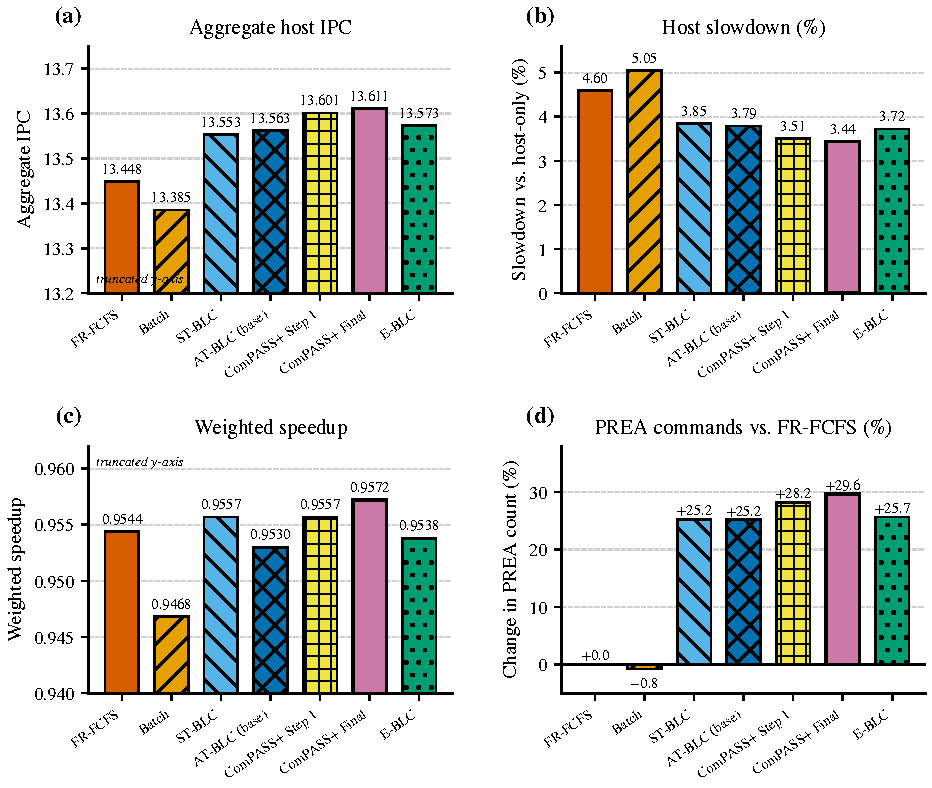
\includegraphics[width=0.82\textwidth]{figs/fig_plus_eval.pdf}
\caption{Modified-simulator results: (a)~aggregate host IPC, (b)~host slowdown, (c)~weighted speedup (y-axes truncated in a, c), (d)~change in PREA count relative to FR-FCFS (positive $=$ more PREA). The ComPASS+ Final bar is outlined.}\label{fig:plus-eval}
\end{figure*}

\Cref{tab:gain} and \cref{fig:plus-gain} quantify the Final configuration against every reference in the same matrix.

\begin{table}[!tbp]
\centering
\caption{ComPASS+ Final versus each reference in the same matrix (IPC 13.6115, slowdown 3.44\%).}\label{tab:gain}
\footnotesize
\begin{tabular}{@{}lrrrr@{}}
\toprule
\textbf{Reference} & \textbf{IPC gain} & \textbf{Slowdown} & \textbf{Rel.\ slowdown} & \textbf{PREA}\\
 & (\%) & (pp) & (\%) & (\%)\\
\midrule
FR-FCFS          & $+1.21$ & $-1.16$ & $-25.2$ & $+29.6$\\
Batch            & $+1.69$ & $-1.61$ & $-31.9$ & $+30.7$\\
ST-BLC           & $+0.43$ & $-0.41$ & $-10.6$ & $+3.5$\\
AT-BLC (base)    & $+0.36$ & $-0.35$ & $-9.2$  & $+3.5$\\
ComPASS+ Step 1  & $+0.07$ & $-0.07$ & $-2.0$  & $+1.1$\\
E-BLC            & $+0.28$ & $-0.28$ & $-7.5$  & $+3.1$\\
\bottomrule
\end{tabular}
\end{table}

\begin{figure*}[!t]
\centering
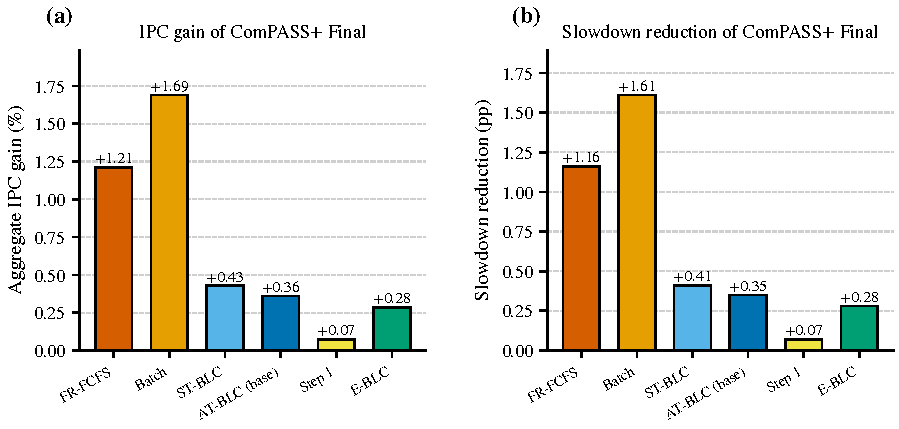
\includegraphics[width=0.8\textwidth]{figs/fig_plus_gain.pdf}
\caption{Gain of ComPASS+ Final over each reference policy: (a)~aggregate IPC gain, (b)~reduction in host slowdown in percentage points.}\label{fig:plus-gain}
\end{figure*}

\paragraph{Summary of the quantities.}
\begin{itemize}
\item Slowdown $3.79\%\to3.44\%$ against the in-matrix AT-BLC baseline ($-0.35$\,pp, $-9.2\%$ relative; the team's notes round this to ``about 10\%''); IPC $13.5627\to13.6115$ ($+0.36\%$); weighted speedup $0.9530\to0.9572$.
\item Against FR-FCFS the host regains 1.21\% IPC and slowdown falls by 25\%.
\item PIM bandwidth is unchanged at 3.12--3.15\,GB/s and all 65{,}536 micro-ops per channel complete.
\item PREA commands rise by 3.5\% over AT-BLC and by 29.6\% over FR-FCFS.
\end{itemize}

\Cref{fig:plus-nt} shows $N(t)$ in the modified controller. The trace begins only after warm-up ($\approx$0.6\,M cycles, I5), enters near 96 and saturates at $N_{\max}=128$ almost immediately, where it stays. Compared with \cref{fig:nadapt}, the early plunge to $N_{\min}$ is gone. Note that after PIM completes (about 0.8\,M cycles per the team's logs) I4 pins $N=N_{\max}$ by design, so the plateau over most of the run reflects surrender rather than ongoing adaptation.

\begin{figure}[!tbp]
\centering
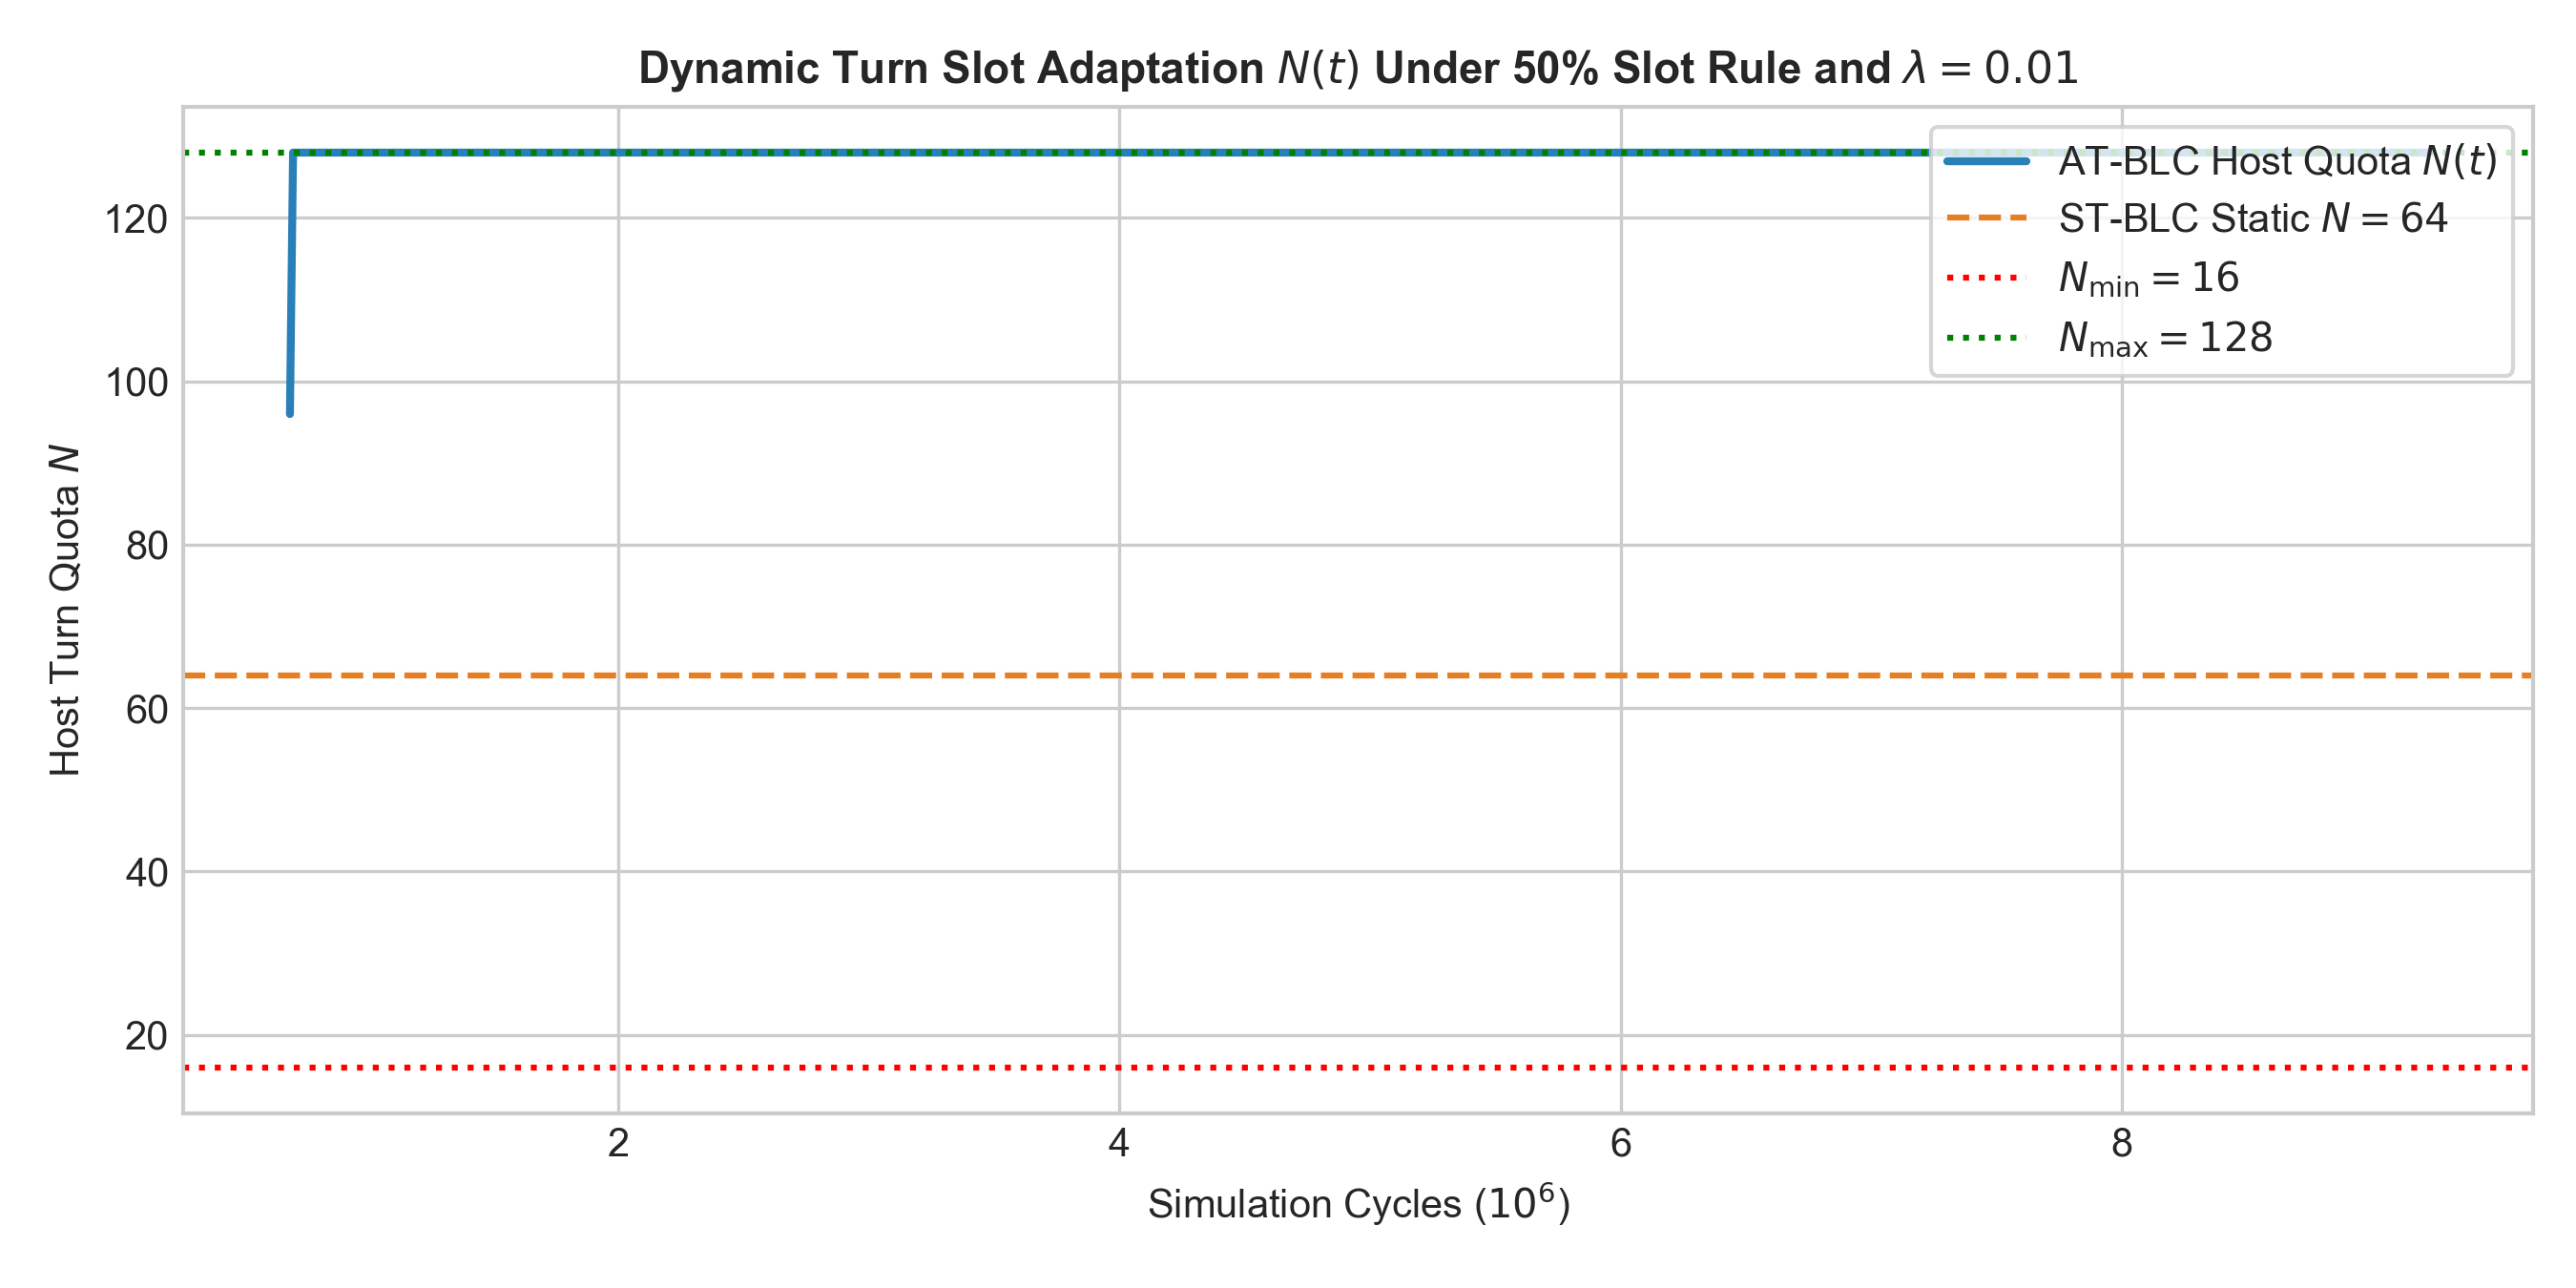
\includegraphics[width=\columnwidth]{figs/plus_Nt.png}
\caption{Host quota $N(t)$ under ComPASS+ (original plot from the team's run). Compare \cref{fig:nadapt}.}\label{fig:plus-nt}
\end{figure}

\subsection{Trade-off Analysis}
\paragraph{PREA count (+3.5\%).} The extra PREAs (151{,}077 $\to$ 156{,}418) follow from longer host bursts: with $N$ reaching 128 instead of sitting at 16, each return to PIM needs a rank-wide precharge, but each PREA now amortises up to 128 host accesses. The net effect is higher IPC, so the added precharges are hidden rather than harmful, in line with ComPASS's goal of overlapping turnaround latency.

\paragraph{Safety margin (10\% $\to$ 5\%).} Relaxation is conditional and reversible: it applies only while PIM is $>5\%$ ahead and reverts in one step if $\delta<-\lambda$. In the team's runs PIM finished in about 0.8\,M cycles against $T=5$\,M with no deadline miss.

\paragraph{PIM bandwidth and hardware cost.} Bandwidth is preserved (3.13$\to$3.14\,GB/s). All changes are integer comparisons, clamps and a bank-index permutation inside the arbiter; no new DRAM pins, commands or tables are required.

\subsection{Design Rationale}
\begin{description}[leftmargin=0pt,labelindent=0pt,font=\bfseries]
\item[Proportional, not maximal, steps.] Jumping straight to $N_{\max}$ would let a host surge stall PIM in the next epoch and swing $N$ back to $N_{\min}$ (chattering). The proportional step, the $\lambda=0.01$ dead band, the 50\% host-utilisation gate, the $[16,128]$ clamp and once-per-$\trefi$ evaluation damp this.
\item[Bank-group striding keeps row locality.] A macro-request still consumes a whole 2\,KB row (64 columns) per activation, so the 98\% row-hit rate is unaffected; only the \emph{next} activation moves to a different bank group, which spreads PIM across independent groups and lowers collisions with host traffic.
\item[Warm-up lock.] During warm-up PIM was disabled, so the rate was zero and $\delta=-1$; dividing by total cycles then kept the rate low even after PIM started. Gating on \cmd{warmup\_complete} and using active-PIM cycles removes this.
\item[Surrender and zero-leak accounting.] Without I4 the turn machine inserts periodic one-cycle bubbles after PIM ends; without I6 an opportunistic fill shortens the next owner's quota.
\item[64-bit parsing.] Linux (LP64) has 64-bit \cmd{unsigned long}; Windows (LLP64) has 32 bits, so 48-bit addresses overflowed. \cmd{stoull} also avoids silent truncation of address bits 32--33 in the 34-bit LPDDR5 map.
\end{description}

\subsection{Critical Assessment and Caveats}\label{sec:plus-caveats}
We report these honestly because they bound what the numbers show.
\begin{enumerate}
\item \textbf{Cross-matrix drift.} Policies that ComPASS+ does not target also moved between our reproduction matrix (\cref{tab:main}) and the modified one (\cref{tab:drift}): FR-FCFS improved by 0.39\,pp, AT-BLC worsened by 0.30\,pp. The $0.35$\,pp gain over the in-matrix AT-BLC is of the same size, so with a single deterministic run per configuration it cannot be cleanly separated from configuration effects.
\item \textbf{Smaller gain against our own AT-BLC.} Against the AT-BLC of \cref{tab:main} (13.6055, 3.49\%) the Final configuration gains only $+0.04\%$ IPC and $-0.05$\,pp slowdown. The headline $\approx$10\% relative gain depends on the weaker in-matrix baseline.
\item \textbf{No ablation.} Only Step~1 $\to$ Final ($-0.07$\,pp) is separable; the individual contribution of I1--I7 is unmeasured.
\item \textbf{Loose QoS target.} PIM completes in about 16\% of $T$, so ``zero violations'' is easily met; the PIM-bandwidth metric divides by total run length and is therefore insensitive to scheduling (3.12--3.15\,GB/s for all policies).
\item \textbf{Unverified code.} The attached \cmd{Controller.cpp} is the upstream Ramulator file (SALP/ALDRAM/TLDRAM specialisations) and does not contain the ComPASS+ changes, which live in \cmd{Controller.h} and \cmd{Processor.cpp}; the mechanisms above are as documented by the team.
\item \textbf{Magnitude.} The $-0.35$\,pp slowdown is small in absolute terms, and PREA commands increase.
\end{enumerate}

\begin{table}[!tbp]
\centering
\caption{Host slowdown (\%) of the same policies in the reproduction matrix (\cref{tab:main}) and in the modified-simulator matrix (\cref{tab:plus}).}\label{tab:drift}
\footnotesize
\begin{tabular}{@{}lrrr@{}}
\toprule
\textbf{Policy} & \textbf{Reproduction} & \textbf{Modified} & \textbf{Shift (pp)}\\
\midrule
FR-FCFS  & 4.99 & 4.60 & $-0.39$\\
Batch    & 4.93 & 5.05 & $+0.12$\\
ST-BLC   & 3.78 & 3.85 & $+0.07$\\
AT-BLC   & 3.49 & 3.79 & $+0.30$\\
E-BLC    & 3.79 & 3.72 & $-0.07$\\
ComPASS+ Final & --- & 3.44 & ---\\
\bottomrule
\end{tabular}
\end{table}

\paragraph{Conclusion of this section.} ComPASS+ fixes real defects (warm-up lock, turn-accounting leak, 64-bit parsing) and gives the lowest slowdown (3.44\%) and highest IPC and weighted speedup of all policies in its matrix at unchanged PIM bandwidth. The margin over the best earlier policy is small (about 0.05--0.35\,pp depending on the baseline), so repeated runs over more trace mixes and a per-feature ablation are the next step before claiming a robust gain.

\appendices
\section{Per-channel Breakdown}\label{app:channel}
\Cref{tab:channel} lists the per-channel statistics behind \cref{fig:baseline-ram}.
\begin{table}[!tbp]
\centering
\caption{Per-channel statistics (PIM requests are 65{,}536 per channel in every run). Host traffic appears only on channels 0 and 2.}\label{tab:channel}
\scriptsize
\setlength{\tabcolsep}{3pt}
\begin{tabular}{@{}llrrrr@{}}
\toprule
\textbf{Policy} & \textbf{Ch} & \textbf{Host req.} & \textbf{PREA} & \textbf{PIM BW (GB/s)} & \textbf{PIM hit (\%)}\\
\midrule
Host-only & 0 & 534{,}416 & 1{,}277 & --- & ---\\
          & 2 & 537{,}011 & 1{,}270 & --- & ---\\
\midrule
FR-FCFS & 0 & 538{,}728 & 59{,}808 & 0.782 & 98.23\\
        & 1 & 0 & 367 & 0.782 & 98.44\\
        & 2 & 541{,}635 & 56{,}110 & 0.782 & 98.18\\
        & 3 & 0 & 367 & 0.782 & 98.44\\
\midrule
Batch   & 0 & 539{,}620 & 56{,}920 & 0.781 & 98.19\\
        & 1 & 0 & 370 & 0.781 & 98.44\\
        & 2 & 541{,}968 & 59{,}365 & 0.781 & 98.21\\
        & 3 & 0 & 370 & 0.781 & 98.44\\
\midrule
\stblc  & 0 & 538{,}872 & 74{,}866 & 0.791 & 98.29\\
        & 1 & 0 & 356 & 0.791 & 98.44\\
        & 2 & 541{,}678 & 77{,}087 & 0.791 & 98.25\\
        & 3 & 0 & 356 & 0.791 & 98.44\\
\midrule
\atblc  & 0 & 541{,}666 & 75{,}036 & 0.781 & 98.26\\
        & 1 & 0 & 356 & 0.781 & 98.44\\
        & 2 & 544{,}456 & 75{,}204 & 0.781 & 98.25\\
        & 3 & 0 & 356 & 0.781 & 98.44\\
\midrule
\eblc   & 0 & 538{,}941 & 75{,}168 & 0.785 & 98.27\\
        & 1 & 0 & 356 & 0.785 & 98.44\\
        & 2 & 541{,}668 & 76{,}071 & 0.785 & 98.26\\
        & 3 & 0 & 356 & 0.785 & 98.44\\
\bottomrule
\end{tabular}
\end{table}

\section{Files Created or Modified}
\Cref{tab:files} lists the principal source files.
\begin{table*}[!t]
\centering
\caption{Principal source files (full manifest in \cmd{PROJECT\_PROGRESS\_AND\_TODO.txt}).}\label{tab:files}
\footnotesize
\begin{tabularx}{\textwidth}{@{}>{\raggedright\arraybackslash}p{6.6cm}>{\raggedright\arraybackslash}X@{}}
\toprule
\textbf{File} & \textbf{Change}\\
\midrule
\multicolumn{2}{@{}l}{\textit{PIMSimulator}}\\
\cmd{BusPacket.h/.cpp} & \cmd{PIM\_ACT} packet, \cmd{isPIM}, \cmd{optype}; constructor bug fix\\
\cmd{PIMCmd.h} & 35-optype ISA, \cmd{NO\_OPTYPE} sentinel\\
\cmd{PIMRank.h/.cpp} & \cmd{doPIMACT}: multi-bank SIMD FP16 execution\\
\cmd{PimActTiming.h} & AAO timing, write-delay calculation, runtime knobs\\
\cmd{CommandQueue.cpp} & all-bank-idle check, PREA-aware scan\\
\cmd{MemoryController.cpp}, \cmd{Rank.cpp} & rank-wide precharge, \cmd{[PIM-REGION]}/\cmd{[MODE-SWITCH]} instrumentation\\
\cmd{tests/KernelTestCases.cpp}, \cmd{PIMKernel.cpp} & four kernels, A3 bitwise verifier\\
\cmd{scripts/analyze\_mode\_switch.py} & mode-switch phase analysis\\
\midrule
\multicolumn{2}{@{}l}{\textit{Ramulator}}\\
\cmd{LPDDR5.h/.cpp}, \cmd{configs/LPDDR5-PIM.cfg} & LPDDR5-6400 model and configuration\\
\cmd{Request.h}, \cmd{Memory.h} & PIM request fields; pending-request accounting\\
\cmd{Controller.h} & \cmd{pim\_q}, request generator, FR-FCFS, Batch, \stblc, \atblc, \eblc, statistics\\
\cmd{Processor.cpp} & CRLF-tolerant trace parser\\
\cmd{evaluate\_policies.py}, \cmd{plot\_results.py}, \cmd{parameter\_sweep.py} & experiment runner, plots, sweep\\
\bottomrule
\end{tabularx}
\end{table*}

% =====================================================================
\begin{thebibliography}{99}
\bibitem{compass} S.~Yu, H.~Kim, K.~Jeun, S.~Hwang, S.~Cho, and E.~Lee, ``ComPASS: A Compatible PIM Protocol Architecture and Scheduling Solution for Processor-PIM Collaboration,'' in \emph{Proc.\ 58th IEEE/ACM Int.\ Symp.\ Microarchitecture (MICRO)}, Seoul, 2025. doi:10.1145/3725843.3756017.
\bibitem{hbmpim} S.~Lee \emph{et al.}, ``Hardware Architecture and Software Stack for PIM Based on Commercial DRAM Technology,'' in \emph{Proc.\ ISCA}, 2021.
\bibitem{aim} M.~He \emph{et al.}, ``Newton: A DRAM-maker's Accelerator-in-Memory (AiM) Architecture for Machine Learning,'' in \emph{Proc.\ MICRO}, 2020.
\bibitem{upmem} F.~Devaux, ``The True Processing In Memory Accelerator,'' in \emph{Hot Chips 31}, 2019.
\bibitem{ramulator} Y.~Kim, W.~Yang, and O.~Mutlu, ``Ramulator: A Fast and Extensible DRAM Simulator,'' \emph{IEEE Computer Architecture Letters}, vol.~15, no.~1, pp.~45--49, 2016.
\bibitem{dramsim2} P.~Rosenfeld, E.~Cooper-Balis, and B.~Jacob, ``DRAMSim2: A Cycle Accurate Memory System Simulator,'' \emph{IEEE Computer Architecture Letters}, vol.~10, no.~1, pp.~16--19, 2011.
\bibitem{rixner} S.~Rixner, W.~J.~Dally, U.~J.~Kapasi, P.~Mattson, and J.~D.~Owens, ``Memory Access Scheduling,'' in \emph{Proc.\ ISCA}, 2000.
\bibitem{parbs} O.~Mutlu and T.~Moscibroda, ``Parallelism-Aware Batch Scheduling: Enhancing both Performance and Fairness of Shared DRAM Systems,'' in \emph{Proc.\ ISCA}, 2008.
\bibitem{lpddr5} JEDEC, \emph{Low Power Double Data Rate 5 (LPDDR5)}, JESD209-5.
\bibitem{spec} J.~L.~Henning, ``SPEC CPU2006 Benchmark Descriptions,'' \emph{ACM SIGARCH Computer Architecture News}, vol.~34, no.~4, 2006.
\bibitem{pimsim} Samsung SAIT, \emph{PIMSimulator}, \url{https://github.com/SAITPublic/PIMSimulator}.
\end{thebibliography}

\end{document}
